\chapter{Tórax}
\subsection{Generalidades de Tórax}
\subsection*{Dosis y Justificación del Estudio}

La radiografía de tórax tiene una dosis efectiva aproximada de 0,1~mSv, equivalente
a unos 10 días de radiación de fondo natural.

El perfil debe incluirse en todo estudio de tórax, dado que aproximadamente el 25\%
del parénquima pulmonar queda oculto en la proyección PA. Las \textbf{excepciones} se
contemplan cuando las condiciones del paciente no permiten realizar el perfil en
condiciones óptimas:

\begin{itemize}
    \item Dificultad de movilidad
    \item Estudios portátiles
    \item Paciente en camilla o silla de ruedas
    \item Preoperatorio
\end{itemize}

\subsection*{Hábito Corporal}

La orientación del chasis varía según el hábito corporal del paciente:

\begin{table}[h]
\centering
\renewcommand{\arraystretch}{1.4}
\begin{tabular}{|l|c|c|}
\hline
\textbf{Hábito corporal} & \textbf{Frecuencia} & \textbf{Orientación del chasis} \\
\hline
Hiperesténico & 5\%  & Horizontal al eje mayor de la región \\
Esténico      & 50\% & Horizontal al eje mayor de la región \\
Hipoesténico  & 35\% & Vertical al eje mayor de la región   \\
Asténico      & 10\% & Vertical al eje mayor de la región   \\
\hline
\end{tabular}
\end{table}

\subsection*{Consideraciones Técnicas}

\subsubsection*{Distancia foco-receptor}

Las radiografías de tórax se realizan a \textbf{180~cm} de distancia foco-receptor,
con el objetivo de minimizar la magnificación de la silueta cardíaca.

\subsubsection*{Parrilla costal}

Para el estudio de la parrilla costal se trabaja a \textbf{100--120~cm}, buscando
desplegar las costillas y resaltar el tejido óseo. La técnica varía según la
localización de las costillas en relación al diafragma:

\begin{itemize}
    \item \textbf{Costillas supradiafragmáticas:} se emplean \textbf{técnicas homogeneizadas},
    dado que el tórax constituye una región de alto contraste intrínseco.
    \item \textbf{Costillas infradiafragmáticas:} se emplean \textbf{técnicas más contrastadas} (NO técnica contrastada a menos que el paciente lo amerite),
    ya que por debajo del diafragma el contraste intrínseco es bajo, en relación
    con el contexto abdominal.
\end{itemize}

\subsection*{Consideraciones sobre el Posicionamiento}

El paciente debe colocarse en \textbf{bipedestación} siempre que sea posible. Esta
posición permite que la gravedad haga descender el diafragma y evita la ingurgitación
de los vasos pulmonares, favoreciendo además la visualización de niveles hidroaéreos.

En \textbf{decúbito}, la gravedad desplaza las vísceras abdominales hacia arriba,
elevando el diafragma y modificando la morfología del campo pulmonar.

En cuanto al \textbf{perfil}, se realiza preferentemente del \textbf{lado izquierdo}
para minimizar la magnificación cardíaca. Cuando la patología se localiza en el
hemitórax derecho, se indica el perfil derecho.

\clearpage

% ============================================================
%  torax.tex
% ============================================================

\subsection{Tórax Frente PA}

\subsubsection*{1. Identificación}
\textbf{Tipo:} Proyección básica estándar. Forma par con la Proyección Lateral de Tórax.\\

\textbf{Indicaciones clínicas principales:}

\begin{itemize}
  \item Neumonía, bronquitis y otras infecciones del tracto respiratorio inferior
  \item Neumotórax (se complementa con proyección en espiración forzada)
  \item Evaluación de silueta cardiaca: cardiomegalia, derrame pericárdico
  \item Derrame pleural y engrosamiento pleural
  \item Lesiones mediastínicas y masas pulmonares
  \item Control post-quirúrgico, post-intubación y seguimiento de patologías crónicas
\end{itemize}

\subsubsection*{2. Técnica Base}

\textbf{Receptor de imagen:} 35 × 43 cm. Orientación \textbf{transversal} en paciente hiperesténico y esténico; \textbf{longitudinal} en asténico e hipoesténico. Borde superior 4 a 5 cm por encima de los hombros.

\textbf{DFRI:} 180 a 200 cm. La distancia larga minimiza la magnificación de estructuras mediastínicas por divergencia del haz y optimiza la radioprotección.

\textbf{Técnica:} Ultra homogeneizada (5 o 6 homogenizaciones). Produce una escala de grises larga que permite visualizar simultáneamente trama pulmonar, mediastino y estructuras óseas, minimizando el contraste innecesario y la dosis al paciente.

\textbf{Factores técnicos:} kVp \textbf{110} — mAs \textbf{2,5}. El espesor se mide a los \textbf{2/3 del tórax} (plano de los pechos). Fórmula base: mAs = 10 × 3,24 × 3,5 $\approx$ 114, dividido sucesivamente por 2 al aplicar cada homogenización. La pérdida de mAs se compensa con el Bucky y la mayor DFRI.

\textbf{Bucky:} Bucky mural con grilla antidifusora.

\subsubsection*{3. Posicionamiento}

\subsubsection*{Paciente}
Bipedestación o sedestación. Plano medio sagital perpendicular al receptor de imagen y centrado en su línea media. Siempre en PA: el corazón y el mediastino quedan cerca del receptor reduciendo su magnificación, y se protegen órganos radiosensibles (tiroides, tejido mamario, esternón). Ambos pies bien apoyados y separados. La posición de pie desciende el diafragma por gravedad, evita la ingurgitación vascular pulmonar y permite demostrar niveles hidroaéreos.

\begin{figure}[h]
    \centering
    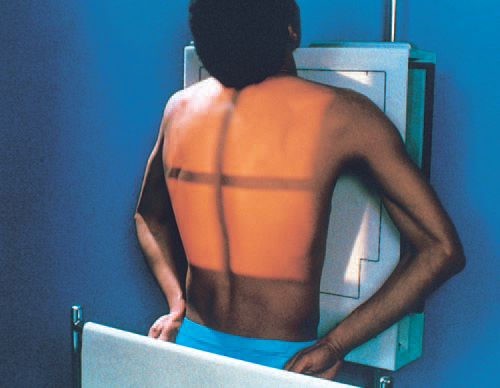
\includegraphics[width=1\linewidth]{imagenes/torax position.png}
    \caption{Posición del paciente}
    \label{fig:1}
\end{figure}

\subsubsection*{Región de interés}
Hombros descendidos y en contacto firme con el receptor, ambos en el mismo plano transversal. Brazos en jarra con el dorso de las manos sobre las caderas y los codos orientados hacia el receptor, lo que rota internamente los húmeros y desplaza las escápulas fuera de los campos pulmonares. Mentón extendido levemente hacia arriba para no bloquear vías aéreas ni vértices. En pacientes con mamas voluminosas, pedirle que las eleve y separe lateralmente para despejar las bases pulmonares.

\subsubsection*{Rayo Central}
Perpendicular al plano del receptor (0°). Punto de entrada: \textbf{T7}, usando el ángulo inferior de las escápulas como reparo anatómico.

\subsubsection*{Receptor de imagen}
Centrado en T7. Borde superior 4 a 5 cm por encima de los hombros para incluir los vértices. El plano medio sagital del paciente coincide con la línea media del receptor.

\subsubsection*{Respiración}
Inspiración forzada máxima, sostenida durante la exposición. Garantiza la máxima expansión del tórax en los tres ejes y el descenso del diafragma. En \textbf{sospecha de neumotórax} se realizan dos exposiciones: una al final de la inspiración forzada y otra al final de la espiración forzada. La comparación evidencia aire libre pleural que puede quedar oculto en inspiración; también demuestra movilidad diafragmática, cuerpo extraño y atelectasia.

\subsubsection*{4. Anatomía Visible}

Tráquea aireada en la línea media. Ambos campos pulmonares completos desde vértices hasta ángulos costofrénico y cardiofrénico. Cúpulas diafragmáticas. Silueta cardiaca y botón aórtico. Trama vascular pulmonar y árbol bronquial. Costillas, clavículas, escápulas (proyectadas fuera de los campos pulmonares) y columna torácica. Las escápulas deben proyectarse fuera de los campos pulmonares. La trama pulmonar debe ser visible a través de la silueta cardiaca. Los ángulos costofrénico y cardiofrénico deben visualizarse íntegros.

\subsubsection*{5. Criterios de Evaluación}

\textbf{Posicionamiento correcto:} campos pulmonares íntegros incluyendo vértices y ángulos costofrénico y cardiofrénico; \textbf{9 a 10 arcos costales posteriores} (horizontales) y \textbf{6 a 7 arcos costales anteriores} (curvos) visibles por encima de las cúpulas diafragmáticas; contornos definidos del corazón y el diafragma; marcas pulmonares visibles desde el hilio hasta la periferia; marca de lado derecho en la imagen.

\textbf{Ausencia de rotación:} extremidades mediales de ambas clavículas equidistantes de la columna vertebral (si la clavícula izquierda parece más corta, el paciente está rotado hacia la izquierda); apófisis espinosas centradas en la línea media; tráquea en la línea media.

\textbf{Penetración y contraste:} trama pulmonar visible a través de la silueta cardiaca, confirmando la técnica ultra homogeneizada. Pulmones, mediastino y estructuras óseas diferenciados en la misma imagen.

\subsubsection*{6. Puntos Críticos}

\textbf{Rotación del paciente:} causa asimetría de clavículas y distorsión de la sombra cardiaca. Corrección: pedir al paciente que adelante el hombro más alejado del Bucky y lo presione contra la superficie hasta que ambos queden en contacto firme y parejo. Si una clavícula aparece más alta, indicarle que al inspirar no eleve los hombros y los relaje en un plano horizontal paralelo al piso.

\textbf{Escápulas superpuestas a los campos:} ocurre cuando los brazos no están en jarra o los codos no se orientan hacia adelante. La rotación interna del húmero es la que desplaza las escápulas.

\textbf{Inspiración insuficiente:} produce menos de 9 costillas posteriores visibles, campos condensados y corazón aparentemente agrandado. El indicador de inspiración correcta es ver 9--10 costillas posteriores y 6--7 anteriores, con trama pulmonar visible a través del corazón.

\textbf{Corte de ángulos costofrénico o cardiofrénico:} pérdida de información diagnóstica crítica. Repetir siempre que sea posible.

\textbf{Adaptaciones:} en paciente que no puede estar de pie, proyección AP en sedestación o decúbito; la mayor magnificación cardiaca es esperada y debe consignarse. Paciente con mamas grandes: elevarlas y separarlas lateralmente. Clavícula congénitamente más alta: no confundir con rotación.

\textbf{Trucos:} el espesor se mide a los 2/3 del tórax, no en el punto más grueso. La DFRI larga compensa la pérdida de mAs de las homogenizaciones; sin esa distancia se pierde nitidez geométrica. Si no se ve trama pulmonar a través del corazón, el kVp o las homogenizaciones fueron insuficientes. La proyección PA magnifica menos el corazón que la AP, dato relevante para medir el índice cardiotorácico.


\begin{figure}[h]
    \centering
    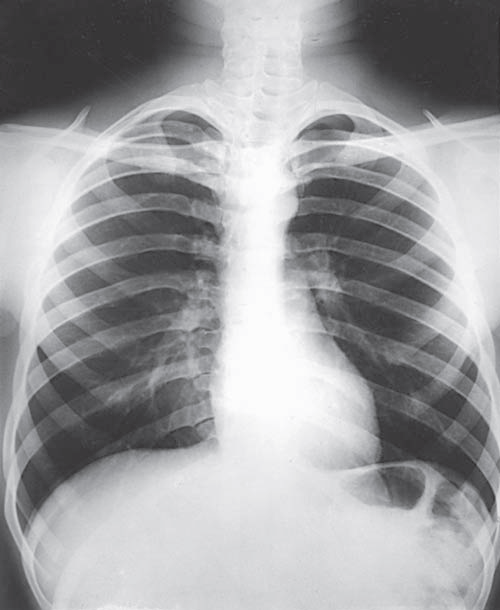
\includegraphics[width=1\linewidth]{imagenes/image.png}
    \caption{Radiografía de Tórax Frente PA}
    \label{fig:2}
\end{figure}

\clearpage

% ============================================================
%  RESUMEN — Proyección Lateral de Tórax (D o I)
% ============================================================

\subsection{Tórax Perfil}

\subsubsection*{1. Identificación}
\textbf{Tipo:} Proyección básica. Forma par con la proyección posteroanterior (PA) de tórax.\\

\textbf{Indicaciones clínicas principales:}

\begin{itemize}
  \item Demostración de patologías situadas por detrás del corazón, grandes vasos y el esternón.
  \item Visualización de fisuras interlobulares y diferenciación de lóbulos pulmonares.
  \item Localización de lesiones pulmonares (complementa la proyección frontal).
  \item Hemotórax (presencia de sangre en cavidad pleural).
  \item Neumotórax (pérdida de trama pulmonar).
\end{itemize}

\subsubsection*{2. Técnica Base}

\textbf{Receptor de imagen:} 35 × 43 cm. Orientación \textbf{longitudinal (vertical)}, con el borde superior ubicado 4 a 5 cm por encima de los hombros.

\textbf{DFRI:} 180 a 200 cm. Distancia aumentada para minimizar la magnificación de las estructuras mediastínicas (reducir la divergencia del haz) y mejorar el detalle óseo de las estructuras torácicas. También contribuye a la radioprotección del paciente.

\textbf{Técnica:} Ultra homogeneizada (5 o 6 homogenizaciones). Permite obtener una escala de grises larga, reduciendo el contraste y posibilitando la visualización simultánea del parénquima pulmonar, el mediastino y las estructuras óseas, incluyendo la trama pulmonar detrás de las costillas y el corazón.

\textbf{Factores técnicos:} kVp \textbf{igual al utilizado en la proyección frontal} — mAs \textbf{= mAs del frente × 4} (factor estándar 3,5; factor 4 en pacientes obesos). El factor de multiplicación compensa el mayor espesor que debe atravesar el rayo central en la proyección lateral.

\textbf{Bucky:} Bucky mural con grilla. Obligatorio dado el espesor de la región y la técnica de alta tensión utilizada.

\subsubsection*{3. Posicionamiento}

\subsubsection*{Paciente}
Paciente en bipedestación o sedestación. El plano medio sagital (PMS) debe quedar paralelo al receptor de imagen. La posición vertical favorece el descenso del diafragma por acción de la gravedad, permitiendo una mejor observación de los campos pulmonares y los ángulos costofrénicos. También facilita la demostración de niveles hidroaéreos y evita la ingurgitación de los vasos sanguíneos pulmonares. El peso corporal debe distribuirse de manera equitativa entre ambas piernas.

\subsubsection*{Región de interés}
El plano medio coronal del paciente se centra en la línea media del receptor. El hombro adyacente al receptor se apoya sobre el mismo. Se le indica al paciente que eleve los brazos por encima de la cabeza, agarrándose los codos entre sí o sosteniéndose de un soporte, con el fin de evitar que las partes blandas de los miembros superiores se superpongan a los campos pulmonares. En pacientes inestables se coloca un soporte auxiliar (gotero u otro elemento de apoyo). Se le indica elevar el mentón y mirar hacia adelante.

\begin{figure}
    \centering
    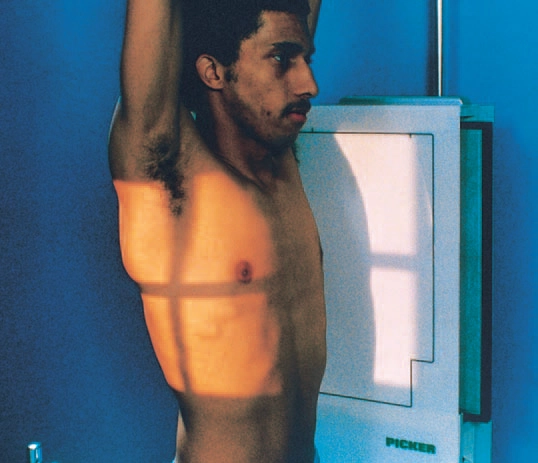
\includegraphics[width=0.75\linewidth]{imagenes/posicion torax perfil.png}
    \caption{Tórax Perfil}
    \label{fig:7}
\end{figure}

\subsubsection*{Rayo Central}
Perpendicular al plano del receptor. Punto de entrada: \textbf{plano medio coronal a la altura de T7 (equivalente al ángulo inferior de las escápulas)}.

\subsubsection*{Receptor de imagen}
Centrado a nivel de T7. El borde superior debe quedar 4 a 5 cm por encima de los hombros para incluir los vértices pulmonares. La región a incluir abarca desde las clavículas hasta los ángulos costofrénicos, incluyendo ambos campos pulmonares y el mediastino completo.

\subsubsection*{Respiración}
Exposición al final de una inspiración forzada (máxima). Garantiza la máxima expansión del tórax en los tres ejes, permitiendo una correcta visualización de los campos pulmonares y los ángulos costofrénicos. Luego del disparo se indica al paciente que retome la respiración con normalidad.

\subsubsection*{4. Anatomía Visible}

Corazón y aorta. Fisuras interlobulares (diferenciación de lóbulos pulmonares). Campos pulmonares en toda su extensión vertical. Mediastino anterior y posterior. Esternón de perfil. Cuerpos vertebrales torácicos con sus espacios intervertebrales y agujeros intervertebrales. Hilios pulmonares (ubicados aproximadamente en el centro de la radiografía). Ángulos costofrénicos. Hemidiafragmas. Arcos costales posteriores superpuestos a la columna vertebral.

\subsubsection*{5. Criterios de Evaluación}

\textbf{Posicionamiento correcto:} Esternón en posición de perfil verdadero. Eje largo de los campos pulmonares demostrado en posición vertical, sin inclinación anterior ni posterior. Ángulos costofrénicos y porción inferior de los vértices pulmonares incluidos. Brazos y partes blandas de los miembros superiores sin superponerse a la porción superior de los campos pulmonares. Hilios ubicados en el centro aproximado de la imagen.

\textbf{Ausencia de rotación:} Arcos costales posteriores superpuestos a los cuerpos vertebrales. El lado alejado del receptor puede aparecer mínimamente por detrás del lado apoyado debido a la divergencia del haz (hallazgo normal). Bordes posteriores de las vértebras visibles como una línea única. Espacios intervertebrales torácicos abiertos y agujeros intervertebrales visualizables (excepto en pacientes con escoliosis). Contornos nítidos del corazón y el diafragma.

\textbf{Penetración y contraste:} Escala de grises larga que permita visualizar simultáneamente el parénquima pulmonar, el mediastino y las estructuras óseas. Penetración adecuada de los campos pulmonares y del corazón.

\subsubsection*{6. Puntos Críticos}

\textbf{Rotación del paciente:} Distorsiona la sombra cardíaca y compromete la correcta evaluación del mediastino. Corrección: recolocar los hombros de modo que el PMS quede paralelo al receptor y el plano medio coronal perpendicular al mismo.

\textbf{Brazos no elevados correctamente:} Las partes blandas de los miembros superiores se superponen a los vértices pulmonares, enmascarando patología. Corrección: indicar al paciente que lleve los brazos bien por encima de la cabeza y que se agarre los codos o se sostenga de un soporte.

\textbf{Adaptaciones:} En pacientes con trauma o imposibilidad de bipedestación se realiza en sedestación o en decúbito lateral con rayo horizontal. En pacientes inestables se utiliza soporte auxiliar (gotero, barra) para mantener la posición de los brazos.

\textbf{Trucos:} La proyección lateral izquierda es el estándar de referencia, ya que el corazón queda más próximo al receptor, minimizando su magnificación y permitiendo una mejor evaluación de la silueta cardíaca. Solo se realiza lateral derecha cuando está específicamente indicado (por ejemplo, para evaluar el pulmón derecho en detalle). El factor de multiplicación de mAs (×4) debe aplicarse siempre respecto a los mAs del frente, no de forma independiente.

\begin{figure}
    \centering
    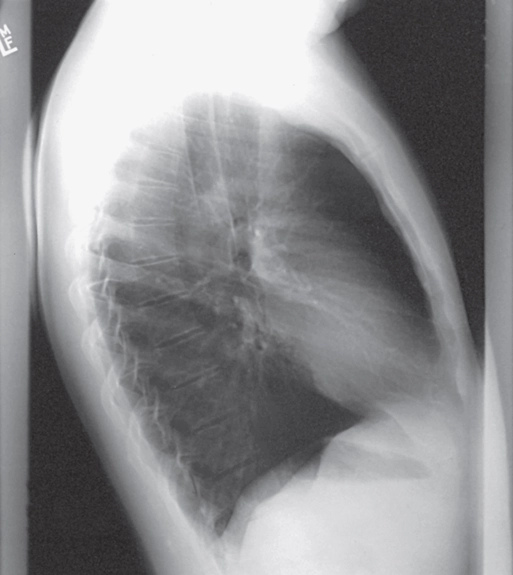
\includegraphics[width=1\linewidth]{imagenes/torax perfil rx.png}
    \caption{Tórax Perfil}
    \label{fig:8}
\end{figure}

\clearpage

\subsection{Anexo de imágenes de tórax}

\begin{figure}[h]
    \centering
    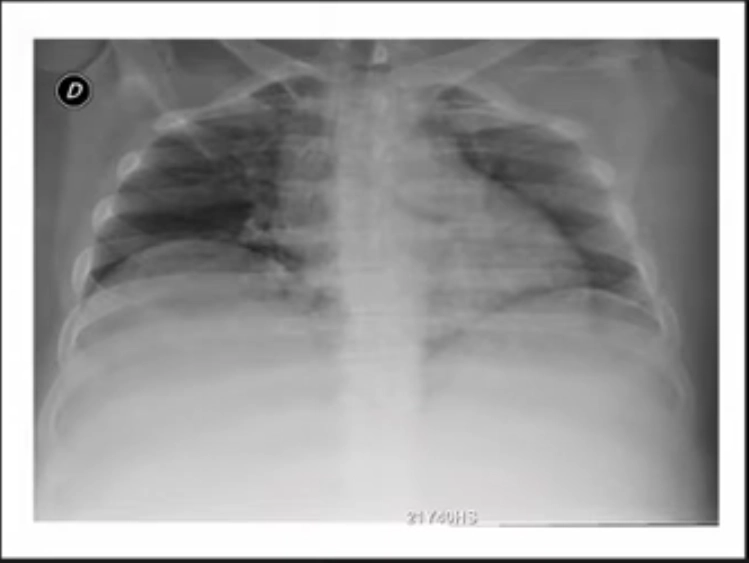
\includegraphics[width=1\linewidth]{imagenes/torax anexo 1.png}
    \caption{Tórax pediátrico}
    \label{fig:87}
\end{figure}

\begin{itemize}
    \item Costillas mas horizontales
    \item Maduración osea de costillas
    \item Glándula timica visible
    \item Probable posición decúbito ya que es pediátrico, ademas la silueta cardíaca esta mas distendida y los vasos pulmonares distendidos.
    \item Marca de la derecha mal posicionada arriba (probablemente).
\end{itemize}

\clearpage

\begin{figure}
    \centering
    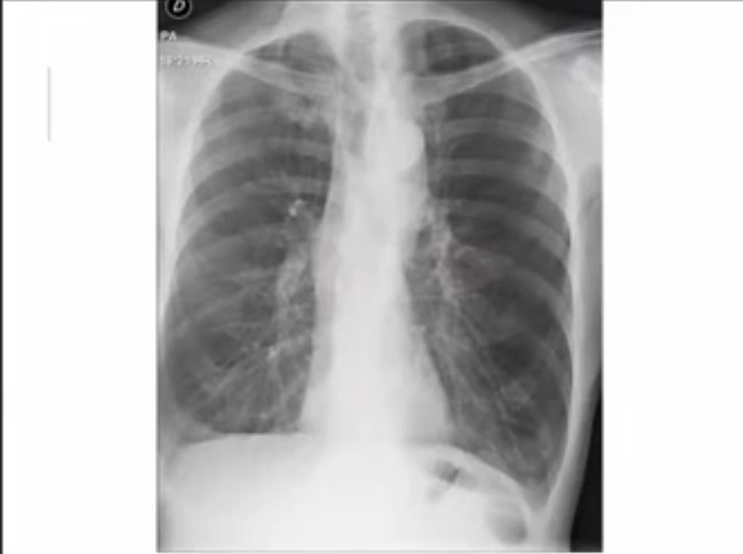
\includegraphics[width=1\linewidth]{imagenes/torax anexo 2.png}
    \caption{Tórax anexo}
    \label{fig:89}
\end{figure}

\begin{itemize}
    \item Paciente adulto Hipoesténico  (5\%).
    \item Uso del chasis en forma \textbf{vertical con respecto al eje mayor de la región} ya que la longitud de los campos pulmonares lo requiere
    \item Pacientes con EPOC (enfermedad pulmonar obstructiva crónica) tienden a tener campos pulmonares mas alargados en el sentido vertical.
    \item La radiografía esta bien inspirada ya que contamos 10 arcos costales.
    \item No tiene valor diagnostico por que esta cortada del lado derecho, parte del campo y el ángulo costo frénico del mismo lado, por ende \textbf{la región no esta comprendida}.    
\end{itemize}

\clearpage

\begin{figure}
    \centering
    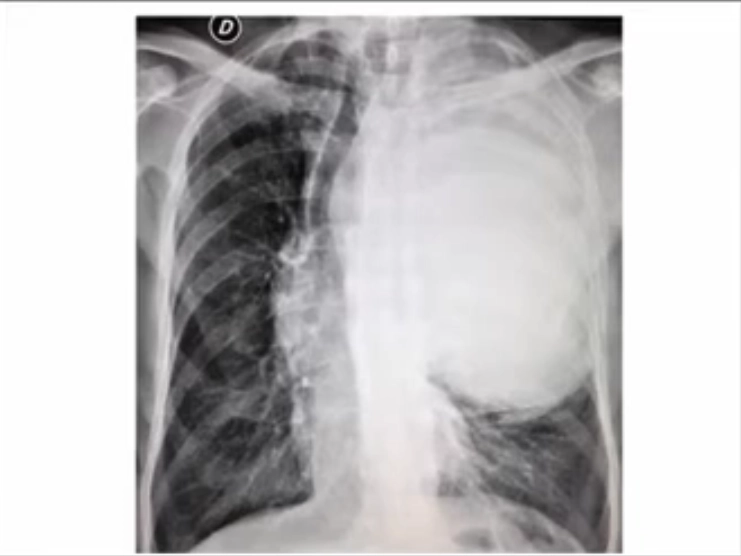
\includegraphics[width=1\linewidth]{imagenes/torax anexo 3.png}
    \caption{Tórax anexo}
    \label{fig:h}
\end{figure}

\begin{itemize}
    \item DC: masa mediastínico.
    \item Los ángulos costofrenicos se encuentran cortados, pero dado que el DC es “masa mediastínica”, por ende \textbf{si tiene valor diagnostico}.
\end{itemize}

\clearpage

\begin{figure}
    \centering
    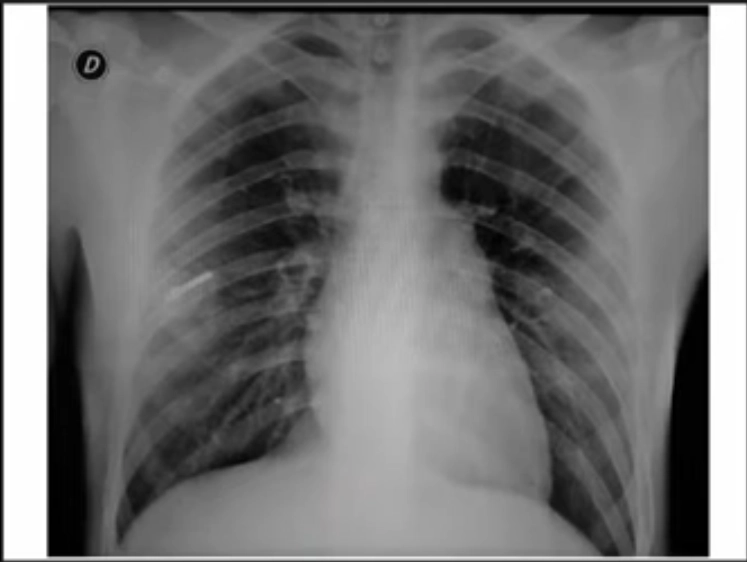
\includegraphics[width=1\linewidth]{imagenes/torax anexo 4.png}
    \caption{Enter Caption}
    \label{fig:766}
\end{figure}

\begin{itemize}
    \item DC: cuerpo extraño en costilla del campo pulmonar derecho
    \item Escapulas dentro del campo pulmonar
    \item Rx bien inspirada ya que contamos 10 costillas posteriores.
    \item No se visualiza el ángulo costofrenicos izquierdo.
    \item No se visualiza del todo el vértice pulmonar derecho
    \item La Rx \textbf{si tiene valor diagnostico} ya que el DC es cuerpo extraño
\end{itemize}

\clearpage

\begin{figure}
    \centering
    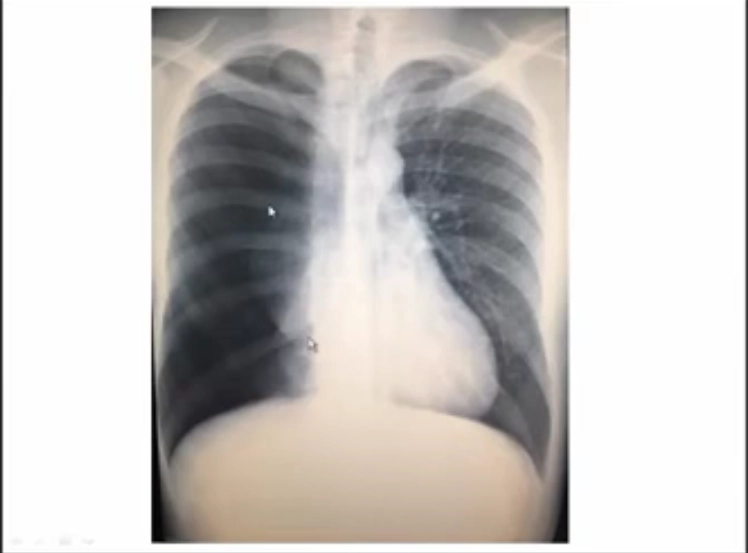
\includegraphics[width=1\linewidth]{imagenes/torax anexo 5.png}
    \caption{Tórax anexo}
    \label{fig:u7uu}
\end{figure}

\begin{itemize}
    \item Rx \textbf{sin valor diagnostico} por falta de marca de la derecha.
    \item Se realizo con el RI en forma vertical con respecto al eje mayor de la región.
    \item Paciente con habito corporal asténico o hipoesténico.
    \item Pulmón derecho sin trama pulmonar, posible neumotórax.
\end{itemize}

\paragraph{Ejercicio:}

DC: Traumatismo costal, dolor en reborde costal derecho superior irradiado hacia adelante.

1. Frente de Tórax PA (SIEMPRE)
2. OAI (para reborde costal) y OPD (para ver mas el reborde esternal) Supra diafragmáticos
3. Técnica en inspiración
4. Técnica intermedia con 2/3 del espesor

\clearpage

% ============================================================
%  RESUMEN — Tórax Portátil (AP)
% ============================================================

\subsection{Tórax - Portátil (Proyección AP)}

\subsubsection*{1. Identificación}
\textbf{Tipo:} Proyección de emergencia/adaptada. Sustituto de la proyección PA estándar cuando el paciente no puede ser trasladado.\\

\textbf{Indicaciones clínicas principales:}

\begin{itemize}
  \item Pacientes críticos o no colaborativos en unidades de cuidados intensivos o sala de internación.
  \item Control de posición de dispositivos médicos (sondas, catéteres, tubo endotraqueal).
  \item Seguimiento de patología torácica en pacientes con imposibilidad de bipedestación.
  \item Sospecha de derrame pleural, neumotórax o consolidación en contexto de urgencia.
\end{itemize}

\subsubsection*{2. Técnica Base}

\textbf{Receptor de imagen:} 35 × 43 cm. Orientación \textbf{transversal} en pacientes hiperesténicos y esténicos; \textbf{longitudinal} en pacientes asténicos e hipoesténicos. La elección se realiza para incluir correctamente el eje longitudinal del tórax según el hábito corporal. Borde superior ubicado 4 a 5 cm por encima de los hombros.

\textbf{DFRI:} La mayor distancia que permita el equipo y la situación. \textbf{Mínima de 100 cm.} A menor distancia se incrementa la magnificación del mediastino; con la distancia habitual de trabajo portátil se genera una magnificación aproximada del 15\% respecto a la proyección PA estándar.

\textbf{Técnica:} Ajustada a la distancia real de trabajo. Sin Bucky, por lo que se debe reducir el kilovoltaje para disminuir la radiación secundaria por efecto Compton y mejorar el contraste de la imagen. La ausencia de grilla genera mayor ruido y menor contraste respecto a la técnica estándar.

\textbf{Factores técnicos:} kVp \textbf{reducido respecto a la técnica estándar} (compensación por ausencia de Bucky). mAs ajustado según la distancia utilizada.

\textbf{Bucky:} No disponible. La ausencia de Bucky es una limitación inherente a la técnica portátil.

\subsubsection*{3. Posicionamiento}

\subsubsection*{Paciente}
Paciente lo más erguido posible, idealmente a 90° en la camilla (sedestación o semisentado). Se indica hacer rodar los hombros hacia adelante, rotando los brazos medial o internamente, para alejar las escápulas de los campos pulmonares. En posición supina o en sedestación son más difíciles de detectar: derrames pleurales (por pérdida del efecto gravitacional), neumotórax (menos evidente que en bipedestación) y niveles hidroaéreos (no se visualizan adecuadamente).

\subsubsection*{Región de interés}
El receptor se coloca detrás del tórax del paciente, alineado respecto al rayo central, con su borde superior 4 a 5 cm por encima de los hombros. Se centra al paciente respecto al rayo central y al receptor. Se recomienda verificar la posición visionando al paciente desde la parte superior, cerca del tubo, para confirmar la alineación.

\begin{figure}
    \centering
    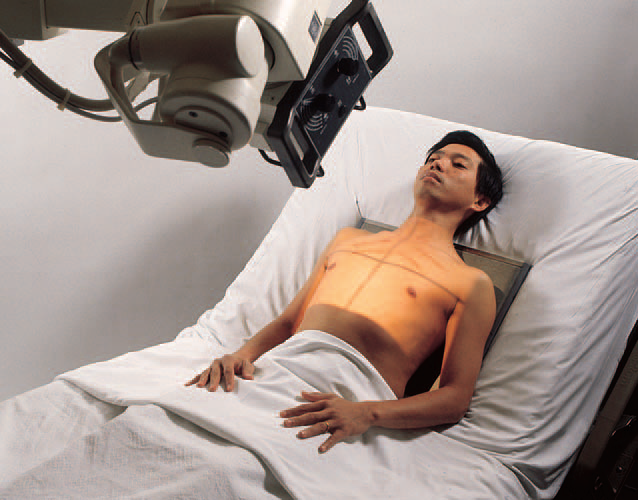
\includegraphics[width=0.75\linewidth]{imagenes/torax portatil.png}
    \caption{Portátil AP de tórax en posición vertical parcial.}
    \label{fig:fhg}
\end{figure}

\begin{figure}
    \centering
    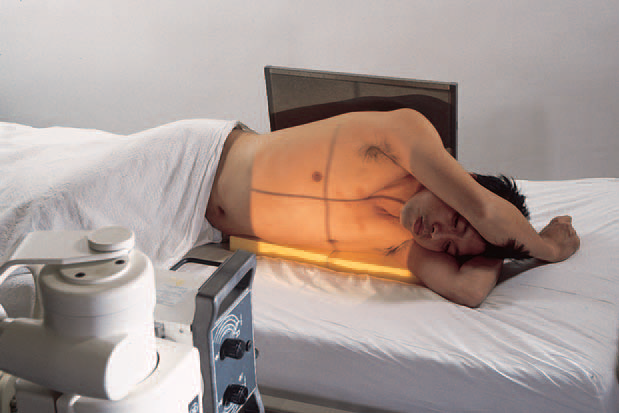
\includegraphics[width=0.75\linewidth]{imagenes/torax portatil .png}
    \caption{Portátil AP de tórax: posición en decúbito lateral izquierdo. Obsérvese el bloque amarillo colocado bajo el tórax para elevarlo. El bloque es necesario para garantizar que el lado izquierdo del tórax quede incluido en la imagen.
}
    \label{fig:lo}
\end{figure}

\subsubsection*{Rayo Central}
Perpendicular al receptor y al esternón como referencia principal. En caso necesario, se angula caudalmente hasta lograr la perpendicularidad respecto al eje longitudinal del esternón (aproximadamente ±5°) para impedir que las clavículas oculten los vértices pulmonares. Punto de entrada: \textbf{T7, aproximadamente 8 a 10 cm por debajo de la escotadura yugular}.

\subsubsection*{Receptor de imagen}
Colocado detrás del tórax del paciente, centrado a nivel de T7. Borde superior 4 a 5 cm por encima de los hombros. Orientación adaptada al hábito corporal del paciente (ver sección Técnica Base).

\subsubsection*{Respiración}
Idealmente suspendida al final de una inspiración completa. Dado que muchos pacientes no pueden colaborar plenamente, se recomienda visualizar el tórax del paciente y disparar en el momento de mayor volumen respiratorio visible.

\subsubsection*{4. Anatomía Visible}

Campos pulmonares. Silueta cardíaca (con magnificación inherente a la técnica). Mediastino. Estructuras óseas torácicas (costillas, clavículas, esternón proyectado). Hemidiafragmas y ángulos costofrénicos (con limitaciones en posición supina). Dispositivos médicos en caso de estar presentes (sondas, catéteres, tubo endotraqueal).

\subsubsection*{5. Criterios de Evaluación}

\textbf{Posicionamiento correcto:} Escápulas alejadas de los campos pulmonares. Tórax centrado respecto al receptor. Clavículas simétricas respecto a la línea media. Inclusión de ambos ángulos costofrénicos y vértices pulmonares.

\textbf{Ausencia de rotación:} Simetría de las clavículas y de las articulaciones esternoclaviculares respecto a la columna vertebral. Columna vertebral centrada en la imagen.

\textbf{Penetración y contraste:} Los mismos criterios de valor diagnóstico que en la radiografía estándar deben mantenerse como objetivo. Se aceptan las siguientes variaciones inherentes a la técnica: (1) silueta cardíaca magnificada como consecuencia del menor DFRI y del aumento de la distancia objeto-receptor; (2) posible ocultamiento de la trama vascular por derrame pleural, más frecuente en esta posición; (3) probable visualización de solo 8 a 9 costillas posteriores por inspiración incompleta, con pulmones de mayor densidad aparente al no estar completamente ventilados.

\subsubsection*{6. Puntos Críticos}

\textbf{Magnificación del mediastino:} Consecuencia directa del menor DFRI y de la proyección AP (mayor distancia objeto-receptor del corazón). No es un error técnico; debe consignarse en el informe y tenerse en cuenta al evaluar el índice cardiotorácico.

\textbf{Ausencia de Bucky:} Genera mayor ruido y menor contraste. No puede evitarse en la técnica portátil; se compensa reduciendo el kVp para disminuir la radiación secundaria por efecto Compton.

\textbf{Adaptaciones:} En pacientes en decúbito supino estricto se realizará la proyección en esa posición, asumiendo las limitaciones diagnósticas para derrame pleural, neumotórax y niveles hidroaéreos. En pacientes con múltiples dispositivos médicos se debe solicitar ayuda al personal del área para posicionar el receptor sin desconectar ni traccionar los mismos.

\textbf{Trucos:} La calidad de imagen de una radiografía portátil nunca debe aceptarse como inferior por el solo hecho de ser portátil; el objetivo sigue siendo alcanzar los mismos criterios diagnósticos de la proyección estándar dentro de las limitaciones del contexto. Visualizar el tórax del paciente desde arriba (cerca del tubo) antes de disparar permite verificar la alineación sin necesidad de movilizar al paciente.

\begin{figure}
    \centering
    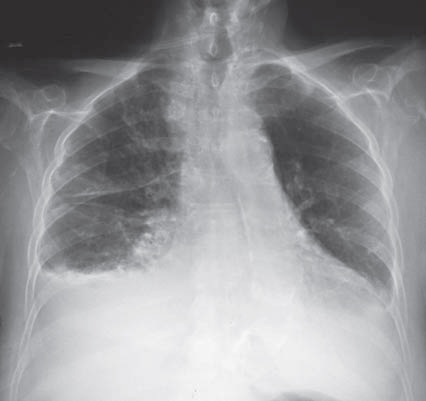
\includegraphics[width=1\linewidth]{imagenes/torax portatil 2.png}
    \caption{Enter Caption}
    \label{fig:7u

\clearpage

% ============================================================
%  PLANTILLA — Resumen de Enfoque Radiológico
% ============================================================

\subsection{Torax - Vértices Pulmonares}

\subsubsection*{1. Identificación}
\textbf{Tipo:} Proyección complementaria. Proyección AP Axial (Método de Lindblom / Posición Lordótica)\\

\textbf{Indicaciones clínicas principales:}

\begin{itemize}
  \item Tuberculosis pulmonar (bacilo de Koch) y sospecha de focos apicales
  \item Nódulos, masas o tumores en vértices pulmonares
  \item Casquetes apicales y calcificaciones en la región de los vértices
  \item Descartar patología pulmonar superior no visible en proyección PA convencional por superposición clavicular
\end{itemize}

\subsubsection*{2. Técnica Base}

\textbf{Receptor de imagen:} 35 × 43 cm. Orientación \textbf{longitudinal}, con el borde superior del chasis ubicado 7--8 cm por encima de los hombros. Se colima \textbf{exclusivamente a los vértices pulmonares}, ya que es un estudio complementario.

\textbf{DFRI:} 180 cm. Igual que en tórax convencional, para reducir la magnificación del corazón y estructuras mediastínicas.

\textbf{Técnica:} Ultra homogeneizada, igual que en tórax PA. Debe ser \textbf{ligeramente mayor} que en la PA convencional, dado el mayor espesor del tórax en posición oblicuada, que requiere mayor penetración para visualizar tejido pulmonar retroóseo (detrás de costillas, clavícula y columna).

\textbf{Bucky:} Bucky de pared con grilla, dado el espesor de la región.

\subsubsection*{3. Posicionamiento}

\subsubsection*{Paciente}
Bipedestación. Plano medio sagital perpendicular al receptor. Posición AP: el paciente apoya la espalda sobre el Bucky de pared. Se le solicita que dé un paso hacia adelante y se deje caer lentamente hacia atrás, apoyando hombros, cuello y nuca contra el Bucky, manteniendo los pies fijos en el piso a unos 30 cm del receptor.

\subsubsection*{Región de interés}
Ambas manos sobre las caderas con las palmas hacia afuera y los hombros proyectados hacia adelante. El dorso de las escápulas queda en contacto con el receptor. Esta hiperextensión del tórax proyecta las clavículas hacia arriba, liberando los vértices pulmonares de su superposición.

\begin{figure}[h]
    \centering
    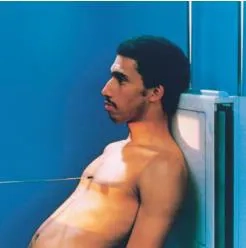
\includegraphics[width=0.5\linewidth]{imagenes/torax vertices.png}
    \caption{Lindblom}
    \label{fig:3}
\end{figure}

\begin{figure}[h]
    \centering
    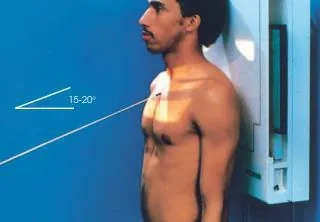
\includegraphics[width=0.5\linewidth]{imagenes/torax vertices 2.png}
    \caption{Lindblom alternativo}
    \label{fig:kifk}
\end{figure}
\clearpage

\subsubsection*{Rayo Central}
\textbf{Opción preferida (paciente apto):} Perpendicular al plano del receptor. Punto de entrada: \textbf{zona media del esternón}.\\
\textbf{Opción alternativa (paciente no logra lordosis):} Angulado \textbf{15--20° en sentido cefálico (craneal)}, centrado en el \textbf{manubrio esternal}. Este ángulo eleva proyectivamente las clavículas, despejando los vértices. Desventaja: produce distorsión de la región. Regla general: \textbf{siempre evitar angular cuando sea posible}.

\subsubsection*{Receptor de imagen}
Centrado en los vértices pulmonares. Borde superior 7--8 cm por encima de los hombros. \textbf{Colimar exclusivamente a los vértices}, sin necesidad de incluir la totalidad de los campos pulmonares.

\subsubsection*{Respiración}
Inspiración máxima para expandir los pulmones y maximizar la visualización del tejido pulmonar apical.

\subsubsection*{4. Anatomía Visible}

Vértices pulmonares bilaterales libres de superposición clavicular. Clavículas proyectadas por encima de los vértices en disposición horizontal. Primeras y segundas costillas con sus extremos mediales superpuestos a los extremos mediales de las clavículas. Segmentos anterior y posterior de las costillas superpuestos y distorsionados por la oblicuación del tórax. Región apical del parénquima pulmonar despejada para evaluar nódulos, infiltrados o calcificaciones.

\subsubsection*{5. Criterios de Evaluación}

\textbf{Posicionamiento correcto:} Clavículas situadas por encima de los vértices pulmonares, sin superponerse sobre el tejido pulmonar apical.

\textbf{Ausencia de rotación:} Extremos esternales (mediales) de ambas clavículas equidistantes respecto a la columna vertebral. Clavículas en disposición horizontal y simétrica.

\textbf{Penetración y contraste:} Técnica ultra homogeneizada que permita visualizar el tejido pulmonar a través de la densidad ósea superpuesta (costillas, columna). Los segmentos anteriores y posteriores de las costillas deben verse distorsionados y superpuestos, confirmando la correcta posición lordótica.

\subsubsection*{6. Puntos Críticos}

\textbf{Paciente no logra la posición lordótica:} Las clavículas permanecen superpuestas a los vértices. Corrección: angular el RC 15--20° en sentido cefálico, centrando en el manubrio. Considerar que esto introduce distorsión geométrica de la región.

\textbf{Colimación excesiva:} Incluir la totalidad de los campos pulmonares implica irradiación innecesaria del paciente. Al ser proyección complementaria (el paciente ya posee frente y perfil), la colimación debe restringirse a los vértices.

\textbf{Técnica insuficiente:} La oblicuación del tórax aumenta el espesor efectivo; si se aplica la misma técnica que en PA convencional, el resultado será una imagen sobreexpuesta en densidad ósea e hipoexpuesta en parénquima. Aumentar levemente los mAs respecto a la PA.

\textbf{Adaptaciones:} En pacientes con dolor torácico agudo o limitación de movilidad, optar directamente por la angulación del RC (15--20° cefálico) sin forzar la posición lordótica. En proyección AP con RC angulado cefálico, las clavículas ascienden. En PA con RC angulado caudal, el resto de las estructuras desciende y las clavículas quedan por encima de los vértices.

\textbf{Trucos:} La posición lordótica es difícil para pacientes con dolor; anticipar la angulación del RC como plan de contingencia. Recordar la regla práctica: AP frente al tubo → ángulo craneal para elevar clavículas; PA → ángulo caudal para el mismo efecto.

\begin{figure}[h]
    \centering
    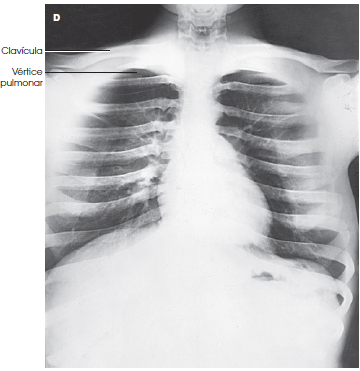
\includegraphics[width=0.5\linewidth]{imagenes/torax vertice 3.png}
    \caption{Se podría colimar mas esta Rx, considerando que ya tiene un frente y perfil de tórax.}
    \label{fig:56}
\end{figure}

\clearpage

% ============================================================
%  Resumen de Enfoque Radiológico
%  Corazón y Grandes Vasos — Proyecciones Oblicuas Anteriores
% ============================================================

\subsection{Tórax - Oblicuas de Corazón y Grandes Vasos (OAD / OAI)}

% ──────────────────────────────────────────────
\subsubsection*{1. Identificación}

\textbf{Tipo:} Proyecciones complementarias entre sí. La OAD y la OAI forman par; ambas se realizan
conjuntamente según la indicación clínica y siempre en proyección PA (anteriores.\\

\textbf{Regla fundamental:} \textbf{Solo se realizan oblicuas anteriores} para corazón y grandes vasos.
Las oblicuas posteriores están contraindicadas porque aumentan la magnificación del mediastino
(la estructura queda alejada del RI) y exponen la cara anterior del tórax del paciente al haz
primario. Si en un examen se pregunta si se realiza una oblicua posterior para corazón
→ \textbf{FALSO}.\\

\textbf{Nomenclatura:} Las oblicuas se nombran según el lado del cuerpo que se apoya contra el RI:

\begin{tcolorbox}[colback=red!5!white, colframe=red!80!black, fonttitle=\bfseries, title=Importante]
\begin{itemize}
  \item \textbf{OAD} (Oblicua Anterior Derecha): hombro anterior derecho apoyado en el RI.
  \item \textbf{OAI} (Oblicua Anterior Izquierda): hombro anterior izquierdo apoyado en el RI.
\end{itemize}
\end{tcolorbox}

\textbf{Principio de visualización:} El lado de \textit{interés diagnóstico} es el más \textbf{alejado} del RI.
Por ello, para visualizar mejor la hemitórax izquierda (cayado aórtico, campo pulmonar izquierdo)
se usa OAI; para visualizar mejor la hemitórax derecha se usa OAD.\\

\textbf{Indicaciones clínicas principales:}

\begin{itemize}
  \item Estudio del corazón y grandes vasos en bloque quirúrgico (procedimientos vasculares:
        control de stent, malla endovascular, aorta).
  \item Esofagograma y estudio gastroduodenal con contraste baritado (para desplegar el esófago
        retrocardiaco y separarlo del mediastino).
  \item Valoración del cayado aórtico y la aorta descendente (preferentemente OAI).
  \item Evaluación del campo pulmonar completo libre de superposición cardiaca o columnar.
  \item Estudio del mediastino en general: separar la columna vertebral de las estructuras
        mediastínicas superpuestas en el frente PA estándar.
\end{itemize}

% ──────────────────────────────────────────────
\subsubsection*{2. Técnica Base}

\textbf{Receptor de imagen:} 35 × 43 cm. Orientación \textbf{longitudinal} (eje mayor vertical),
independientemente del hábito corporal del paciente, para incluir todo el tórax desde los vértices
pulmonares hasta los ángulos costofrénicos.\\

\textbf{Posición del RI:} El borde superior se sitúa \textbf{4--5 cm por encima de C7} (vértebra
prominente) para asegurar la inclusión completa de los vértices.\\

\textbf{DFRI:} \textbf{180 cm}. La distancia foco-receptor incrementada disminuye la magnificación
de las estructuras mediastínicas (el corazón y los grandes vasos se ubican a distancia del RI en
proyección PA), mejorando la nitidez geométrica y la fidelidad de tamaño.\\

\textbf{Técnica:} Ultra-homogeneizada en paciente delgado, con \textbf{alto kVp} (escala larga de
grises). Este ajuste técnico es imprescindible para visualizar simultáneamente el parénquima
pulmonar, las estructuras mediastínicas y la silueta cardiaca, que de otro modo quedarían
enmascaradas por superposición ósea y la densidad cardiaca.

\begin{itemize}
  \item En pacientes con mucha grasa (obesos): técnica intermedia, mayor radiación dispersa,
        puede requerirse incremento de mAs controlado.
  \item Para visualización de stent o malla metálica: se prioriza la transparencia, con kVp
        muy alto para ``atravesar'' la densidad cardiaca y revelar el metal con claridad.
\end{itemize}

\textbf{Bucky:} Sí. Se utiliza bucky mural (vertical) con grilla, dada la profundidad del tórax y
la producción de radiación dispersa significativa.\\

\textbf{Importante sobre radioprotección:} Al ser proyecciones en PA (paciente de espaldas al tubo),
el haz entra por la espalda, protegiendo las estructuras radiosensibles anteriores
(cristalino, tiroides, gónadas). La radioprotección es un criterio de elección activo para estas
proyecciones.

% ──────────────────────────────────────────────
\subsubsection*{3. Posicionamiento}

\subsubsection*{Paciente}

Paciente en \textbf{bipedestación} (de pie) o, si no es posible, sentado erguido. Posición PA:
el tórax enfrenta el RI, la espalda queda dirigida hacia el tubo de rayos X.

\subsubsection*{Región de interés}

Rotación del tórax sobre su eje longitudinal, alejando el lado de interés del RI:

\begin{itemize}
  \item \textbf{45° de rotación} para el estudio del \textbf{pulmón}.
  \item \textbf{60° de rotación} para el estudio del \textbf{corazón y grandes vasos}.
\end{itemize}

La angulación se mide desde el plano frontal del paciente.

\textbf{OAD:} Se aleja el hombro izquierdo del RI; el hombro anterior derecho queda apoyado.\\
\textbf{OAI:} Se aleja el hombro derecho del RI; el hombro anterior izquierdo queda apoyado.\\

Posición de los miembros superiores:

\begin{itemize}
  \item \textbf{Del lado apoyado:} la mano se coloca sobre la cadera con la palma hacia afuera,
        alejando el brazo del campo pulmonar.
  \item \textbf{Del lado alejado:} el paciente eleva el brazo hasta la altura del hombro y apoya
        la mano sobre la cabeza, evitando que el miembro superior tape el campo pulmonar contralateral.
  \item Variante: tomarse los codos por encima de la cabeza (ambos brazos elevados).
  \item Los hombros deben quedar en un mismo plano horizontal para evitar rotación asimétrica.
  \item El paciente no debe rotar la cabeza: mirar hacia adelante con el mentón elevado.
\end{itemize}

\subsubsection*{Rayo Central}

RC \textbf{perpendicular} al plano del RI (sin angulación).

\begin{itemize}
  \item \textbf{OAD:} el RC incide a nivel del ángulo inferior de la escápula \textbf{izquierda}
        (la escápula del lado alejado, que corresponde al centro del campo de interés proyectado).
  \item \textbf{OAI:} el RC incide a nivel del ángulo inferior de la escápula \textbf{derecha}.
  \item Referencia alternativa equivalente: \textbf{T7}, aproximadamente 8--10 cm por debajo
        de la escotadura yugular (medido a nivel de la vértebra prominente C7).
\end{itemize}

\subsubsection*{Receptor de imagen}

Centrado respecto al eje del tórax del paciente, con borde superior 4--5 cm por encima de C7.
El campo debe incluir:

\begin{itemize}
  \item \textbf{Ambos pulmones} en su totalidad: desde los vértices pulmonares hasta los ángulos
        costofrénicos inferiores.
  \item Estructuras mediastínicas completas (tráquea, cayado aórtico, silueta cardiaca).
\end{itemize}

\subsubsection*{Respiración}

\textbf{Inspiración máxima sostenida} (``Respire hondo y aguante el aire''). La inspiración profunda
desciende el diafragma, expande los campos pulmonares y aumenta el contraste aire/tejido blando,
mejorando la visualización del parénquima y las estructuras vasculares.

\textit{Control de inspiración:} contar los arcos costales posteriores (los más horizontales)
por encima de la cúpula diafragmática. Lo esperado son \textbf{9--10 arcos posteriores}. Si se
observan solo 8, la inspiración fue insuficiente y la proyección debe repetirse.

% ──────────────────────────────────────────────
\subsubsection*{4. Anatomía Visible}

\textbf{En la OAD:}
\begin{itemize}
  \item Silueta cardiaca con morfología \textbf{triangular}.
  \item Aorta ascendente y cayado aórtico \textbf{sin desplegar} (el cayado se proyecta superpuesto
        en OAD; para desplegarlo se usa OAI).
  \item \textbf{Espacio aéreo retroesternal} delante del corazón con morfología triangular.
  \item Tráquea y \textbf{árbol bronquial izquierdo} completo desplegado (tráquea llena de aire
        y carina visible sobre la silueta cardiaca, no sobre la columna).
  \item Cámara gástrica \textbf{alejada} de la columna vertebral (configuración en ``posición de
        esgrimista'').
  \item Campo pulmonar izquierdo visualizado en mayor extensión.
\end{itemize}

\begin{figure}
    \centering
    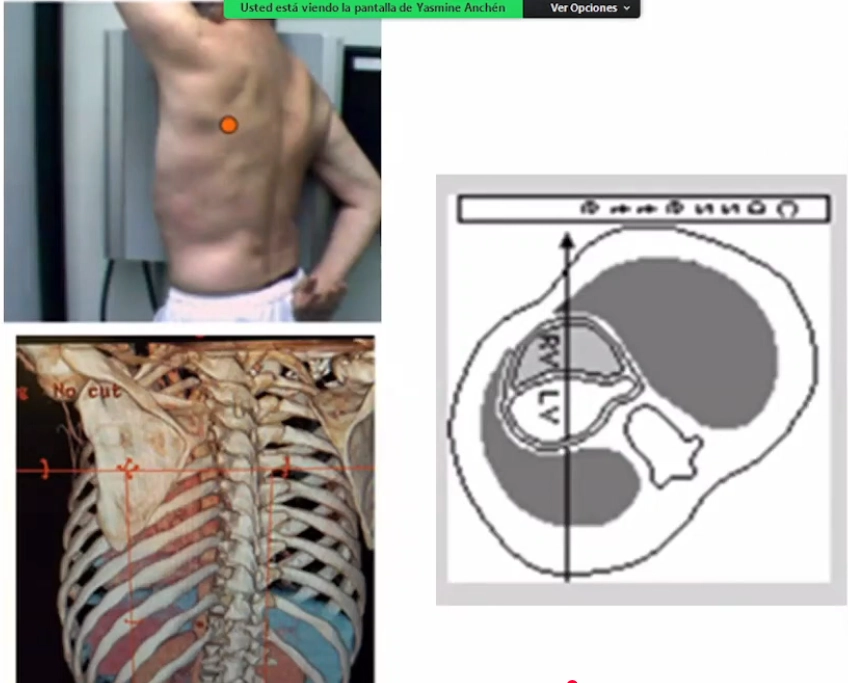
\includegraphics[width=0.65\linewidth]{imagenes/grandes vasos OAD.png}
    \caption{OAD}
    \label{fig:546}
\end{figure}

\begin{figure}
    \centering
    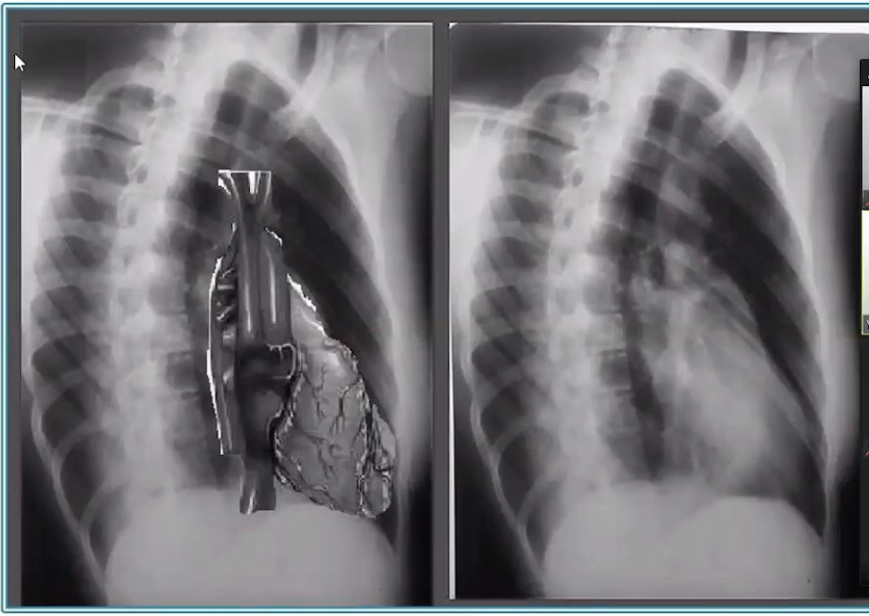
\includegraphics[width=0.65\linewidth]{imagenes/grandes vasos RX OAD.png}
    \caption{OAD}
    \label{fig:4}
\end{figure}

\clearpage

\textbf{En la OAI:}
\begin{itemize}
  \item Silueta cardiaca con morfología \textbf{en pera} (el ventrículo izquierdo se proyecta hacia
        la izquierda inferior).
  \item \textbf{Cayado aórtico desplegado} y nítido (aorta ascendente, cayado y aorta descendente
        separados).
  \item \textbf{Espacio aéreo} delante del corazón con morfología \textbf{rectangular}.
  \item Cámara gástrica más \textbf{próxima} a la columna (configuración en ``posición de
        boxeador'').
  \item Campo pulmonar derecho visualizado en mayor extensión.
  \item Esófago retrocardiaco visible cuando se usa contraste baritado.
\end{itemize}

\clearpage

\begin{figure}
    \centering
    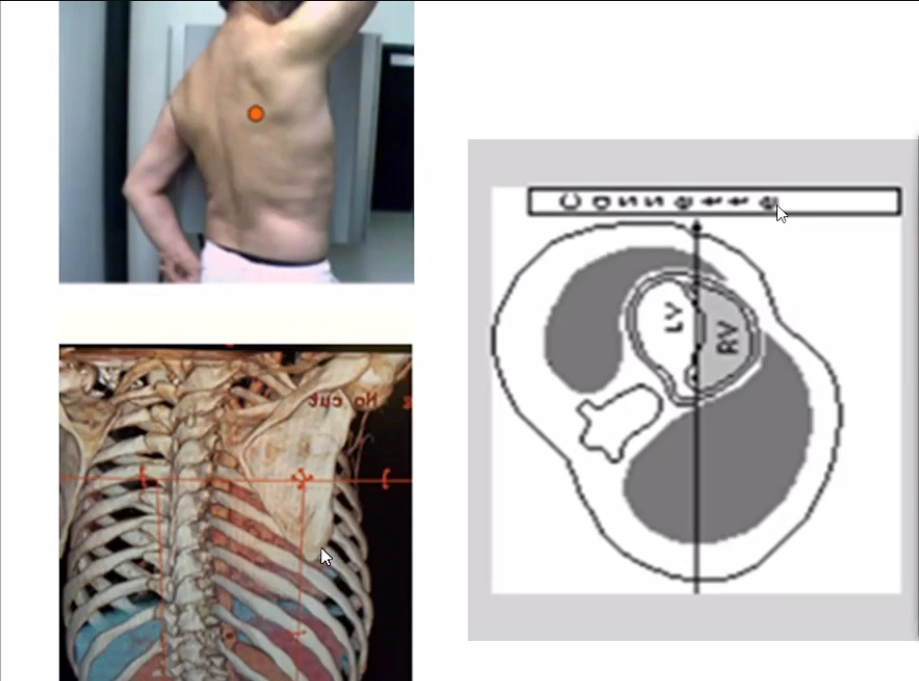
\includegraphics[width=0.65\linewidth]{imagenes/grandes vasos OAI.png}
    \caption{OAI}
    \label{fig:5}
\end{figure}

\begin{figure}
    \centering
    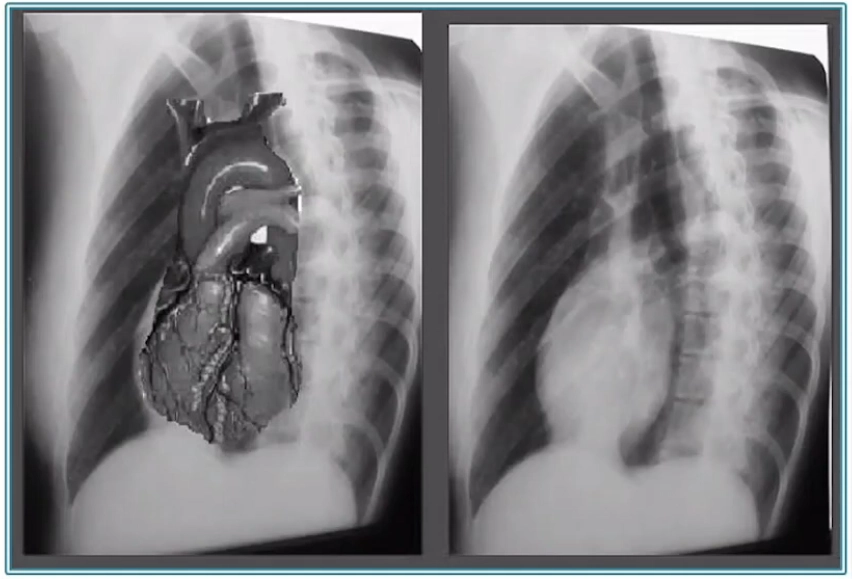
\includegraphics[width=0.65\linewidth]{imagenes/grandes vasos RX OAI.png}
    \caption{OAI}
    \label{fig:6}
\end{figure}

\clearpage
% ──────────────────────────────────────────────
\subsubsection*{5. Criterios de Evaluación}

\textbf{Posicionamiento correcto (OAD):}
\begin{itemize}
  \item Corazón de morfología triangular.
  \item Espacio aéreo anterior triangular delante del corazón.
  \item Cámara gástrica alejada de la columna (``esgrimista'').
  \item Árbol bronquial izquierdo completamente desplegado.
\end{itemize}

\textbf{Posicionamiento correcto (OAI):}
\begin{itemize}
  \item Corazón de morfología en pera.
  \item Cayado aórtico desplegado, aorta ascendente y descendente separadas.
  \item Espacio aéreo anterior rectangular.
  \item Cámara gástrica próxima a la columna (``boxeador'').
\end{itemize}

\textbf{Control de rotación:}
\begin{itemize}
  \item Tráquea llena de aire con perfil nítido.
  \item Bifurcación traqueal (carina) proyectada \textbf{sobre la silueta cardiaca}, no sobre
        la columna vertebral (si la carina cae sobre la columna, la rotación es insuficiente).
  \item Hombros en el mismo plano horizontal.
\end{itemize}

\textbf{Penetración y contraste:}
\begin{itemize}
  \item Escala larga de grises que permita visualizar simultáneamente el parénquima pulmonar
        y el mediastino.
  \item La trama vascular pulmonar debe ser visible hasta la periferia de los campos.
  \item El corazón no debe ser completamente radiopaco: debe poder ``atravesarse''
        ópticamente para evaluar estructuras retrocar\-dia\-cas (especialmente en OAI con bario).
  \item \textbf{9--10 arcos costales posteriores} visibles por encima del diafragma confirman
        inspiración adecuada.
\end{itemize}

% ──────────────────────────────────────────────
\subsubsection*{6. Puntos Críticos}

\textbf{Corazón encimado a la columna (OAI):} Falta de rotación. El hombro derecho no se alejó
lo suficiente del RI. Consecuencia: el mediastino no se despliega y la columna superpone el campo
pulmonar opuesto. Corrección: aumentar la rotación hasta 60°, verificar posición de hombros.\\

\textbf{Columna tapando el campo pulmonar contralateral:} El paciente se colocó demasiado de perfil
(rotación excesiva). Consecuencia: se pierde información del campo pulmonar alejado. Corrección:
reducir el grado de rotación.\\

\textbf{Corazón muy radiopaco sin poder verlo:} Técnica demasiado baja (kVp insuficiente).
Consecuencia: pérdida de información retrocardiaca y mediastínica. Corrección: subir kVp para
obtener escala larga de grises.\\

\textbf{Imagen con apariencia de parrilla costal (sin trama pulmonar visible):} Técnica ósea
aplicada erróneamente. Corrección: usar técnica ultra-homogeneizada con alto kVp.\\

\textbf{Inspiración insuficiente:} Solo 8 arcos costales posteriores visibles. Consecuencia:
los campos pulmonares no se expanden completamente, los ángulos costofrénicos pueden no incluirse
y el contraste aire/tejido disminuye. Corrección: repetir con instrucción clara al paciente
(``respire todo lo que pueda y aguante'').\\

\textbf{Brazo del lado alejado tapando el pulmón:} El paciente no elevó correctamente el miembro
superior del lado alejado. Corrección: indicar que eleve el brazo y apoye la mano sobre la cabeza,
o que tome ambos codos por encima de la cabeza.\\

\textbf{Adaptaciones:} En pacientes con limitación para la bipedestación se puede realizar
en sedestación erguida manteniendo los mismos criterios de posicionamiento. Para procedimientos
en bloque quirúrgico (control de stent o malla) se prioriza alto kVp con escala muy larga
para revelar el material metálico a través de la densidad cardiaca.\\

\textbf{Trucos:}
\begin{itemize}
  \item Para desplegar el cayado aórtico siempre usar OAI. En OAD el cayado queda superpuesto
        y no es valorable.
  \item Para ver el campo pulmonar izquierdo completo sin superposición cardíaca, usar OAI.
  \item Para ver el campo pulmonar derecho completo, usar OAD.
  \item La ``posición del esgrimista'' (cámara gástrica alejada de columna) es el signo
        nemotécnico de OAD correcta; la ``posición del boxeador'' (cámara gástrica próxima a
        columna) es el signo de OAI correcta.
  \item Contar arcos posteriores es más fiable que los anteriores para evaluar la inspiración,
        ya que los arcos posteriores son más horizontales y más fáciles de identificar.
\end{itemize}

\clearpage

% ============================================================
%  Parrilla Costal — Frente
% ============================================================

\subsection{Tórax - Parrilla Costal Frente}

% ------------------------------------------------------------
\subsubsection*{Anamnesis Previa}
% ------------------------------------------------------------

Realizar las siguientes preguntas si no se dispone de historia clínica:

\begin{enumerate}
  \item Naturaleza del traumatismo: dolor agudo o crónico y mecanismo de producción.
  \item Localización del dolor o lesión costal.
  \item Si la lesión fue producida por traumatismo de cavidad torácica (dificultad respiratoria).
  \item Determinar si el paciente puede ponerse de pie antes de iniciar el procedimiento.
\end{enumerate}

\textbf{Protocolo obligatorio de dos pasos en traumatismo:}
\begin{enumerate}
  \item \textbf{Radiografía de tórax PA} — descartar neumotórax o hemotórax.
  \item \textbf{Estudio específico de costillas} según localización del traumatismo.
\end{enumerate}

% ------------------------------------------------------------
\subsubsection*{1. Identificación}
% ------------------------------------------------------------

\textbf{Tipo:} Proyección básica de parrilla costal. Puede realizarse en AP (arcos posteriores) o PA (arcos anteriores) según la región de interés.\\

\textbf{Indicaciones clínicas principales:}

\begin{itemize}
  \item Traumatismo de la caja torácica — sospecha de fractura costal.
  \item Dolor costal agudo o crónico de origen no precisado.
  \item Evaluación de lesiones neoplásicas o metastásicas en arcos costales.
\end{itemize}

\textbf{Clasificación según relación con el diafragma:}

\begin{itemize}
  \item \textbf{Supra diafragmáticas:} por encima del 9° arco costal.
  \item \textbf{Infra diafragmáticas:} del 9° arco costal hacia abajo.
\end{itemize}

% ------------------------------------------------------------
\subsubsection*{2. Técnica Base}
% ------------------------------------------------------------

\textbf{Receptor de imagen:} 35 × 43 cm.\\

\textbf{DFRI:} 100 cm (1 metro).\\

\textbf{Técnica:}
\begin{itemize}
  \item \textbf{Supra diafragmáticas:} homogeneizada o intermedia. Las costillas superiores están rodeadas de tejido pulmonar aireado; un kVp relativamente bajo mantiene el contraste y permite visualizarlas a través del parénquima. Si la lesión está en zona cardíaca, aumentar kVp para penetrar la silueta cardíaca.
  \item \textbf{Infra diafragmáticas:} básica o contrastada. Las costillas inferiores están rodeadas por diafragma muscular y estructuras abdominales densas; se requiere mayor penetración y contraste entre hueso y tejidos blandos.
\end{itemize}

\textbf{Factores técnicos:}
\begin{itemize}
  \item Supra: kVp \textbf{65--70}.
  \item Infra: kVp \textbf{70--80}.
\end{itemize}

\textbf{Bucky:} Bucky mural (bipedestación) o Bucky de mesa (decúbito).

% ------------------------------------------------------------
\subsubsection*{3. Posicionamiento}
% ------------------------------------------------------------

\subsubsection*{\small 3a. Costillas Supra Diafragmáticas}

\paragraph*{Paciente}
Bipedestación. La gravedad hace descender el diafragma a su posición más baja, favorece la inspiración profunda y reduce la presión de la caja torácica, minimizando el dolor por movimiento.

\begin{itemize}
  \item \textbf{Arcos posteriores:} AP — espalda apoyada contra el receptor.
  \item \textbf{Arcos anteriores:} PA — tórax apoyado contra el receptor.
\end{itemize}

Eje medio sagital perpendicular al receptor.

\paragraph*{Región de interés}
Siempre apoyar la región a radiografiar contra el receptor para maximizar el detalle. En estudios unilaterales, centrar en la región de interés.

\paragraph*{Rayo Central}
Perpendicular al plano del receptor.\\
\textbf{Bilateral:} centrado en T7 (mitad del esternón).\\
\textbf{Unilateral:} centrado en la línea medio clavicular del hemitórax afectado.

\paragraph*{Receptor de imagen}
Centrado a nivel de T7 para estudios bilaterales. Borde superior por encima del primer arco costal; borde inferior por debajo del diafragma.

\paragraph*{Respiración}
\textbf{Inspiración profunda.} El diafragma desciende, el campo pulmonar se expande y los arcos costales quedan libres de superposición de partes blandas. El diafragma se proyecta por debajo de la 9ª--10ª costilla en inspiración plena. En lesiones dolorosas puede lograrse solo una inspiración parcial, visualizándose 8--9 costillas posteriores.

\begin{figure}[h]
    \centering
    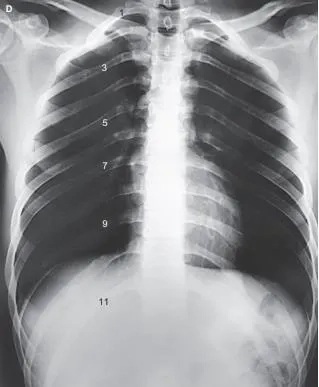
\includegraphics[width=1\linewidth]{imagenes/costilla supra.png}
    \caption{Supra diafragmáticas AP}
    \label{fig:9}
\end{figure}

\clearpage
% ------------------------------------------------------------

\subsubsection*{\small 3b. Costillas Infra Diafragmáticas}

\paragraph*{Paciente}
Decúbito supino. El diafragma se eleva a su posición más alta, reduciendo el espesor abdominal y mejorando la visualización de costillas inferiores a través de las estructuras abdominales.

Eje medio sagital perpendicular al receptor.

\paragraph*{Región de interés}
Siempre apoyar la región a radiografiar contra el receptor.

\paragraph*{Rayo Central}
Perpendicular al plano del receptor.\\
\textbf{Bilateral:} centrado a la altura de la apófisis xifoides.\\
\textbf{Unilateral:} centrado en la línea medio clavicular del lado afectado.

\paragraph*{Receptor de imagen}
Centrado a nivel de la apófisis xifoides para estudios bilaterales. Borde inferior a nivel de las crestas ilíacas.

\paragraph*{Respiración}
\textbf{Espiración.} El diafragma asciende a nivel de la 7ª--8ª costilla posterior, generando una densidad uniforme por debajo de él. Evita la interfase aire/partes blandas que podría simular fracturas.

\begin{figure}[h]
    \centering
    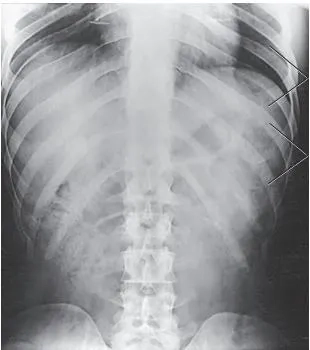
\includegraphics[width=1\linewidth]{imagenes/costillas infra.png}
    \caption{Infra diafragmáticas AP}
    \label{fig:456n}
\end{figure}

\clearpage
% ------------------------------------------------------------
\subsubsection*{4. Anatomía Visible}
% ------------------------------------------------------------

\textbf{Supra diafragmáticas:}
\begin{itemize}
  \item Arcos costales posteriores del 1° al 10° por encima del diafragma, visualizados a través del parénquima pulmonar.
  \item En AP se visualizan preferentemente arcos posteriores; en PA, arcos anteriores con mayor detalle por proximidad al receptor.
  \item La porción cartilaginosa anterior no es visible (a menos que este    calcificada).
\end{itemize}

\textbf{Infra diafragmáticas:}
\begin{itemize}
  \item 11ª y 12ª costillas por debajo del diafragma, a través de estructuras abdominales.
\end{itemize}

\textbf{Nota anatómica:} La mayor cantidad de fracturas ocurre en el \textbf{borde axilar} de los arcos costales, zona no evaluable en el frente simple — requiere proyecciones oblicuas específicas.

% ------------------------------------------------------------
\subsubsection*{5. Criterios de Evaluación}
% ------------------------------------------------------------

\textbf{Posicionamiento correcto — Supra:} arcos costales posteriores del 1° al 10° visibles por encima del diafragma. En exploraciones unilaterales las costillas contralaterales pueden estar incompletas sin pérdida diagnóstica.

\textbf{Posicionamiento correcto — Infra:} costillas 11ª y 12ª visibles por debajo del diafragma; borde inferior de la imagen a nivel de las crestas ilíacas.

\textbf{Ausencia de rotación:} simetría bilateral de estructuras torácicas o abdominales. Eje medio sagital perpendicular verificado por equidistancia de ambos hemitórax.

\textbf{Penetración y contraste:}
\begin{itemize}
  \item \textbf{Supra}: visualización clara de los arcos a través del parénquima pulmonar aireado.
  \item \textbf{Infra}: penetración adecuada de las estructuras abdominales densas con contraste suficiente hueso/tejido blando.
\end{itemize}

% ------------------------------------------------------------
\subsubsection*{6. Puntos Críticos}
% ------------------------------------------------------------

\textbf{Fase respiratoria incorrecta:} en supra diafragmáticas, la espiración eleva el diafragma y superpone costillas con partes blandas; en infra, la inspiración genera interfase aire/tejidos que simula fracturas. Verificar siempre la fase antes de exponer.

\textbf{Omisión de la radiografía de tórax PA previa:} en traumatismos nunca iniciar el estudio de costillas sin descartar primero neumotórax o hemotórax.

\textbf{Adaptaciones:} en pacientes con dolor severo que no toleran bipedestación, las supra pueden realizarse en decúbito; considerar que el diafragma se elevará y se verán menos costillas libres. Las infra pueden realizarse en bipedestación si el paciente no tolera decúbito, aceptando mayor espesor abdominal.

\textbf{Trucos:}
\begin{itemize}
  \item El borde axilar es la zona de mayor incidencia de fractura y no se evalúa en el frente — siempre complementar con oblicuas ante sospecha clínica.
  \item En lesiones costales dolorosas el paciente raramente logra inspiración plena; anticipar que pueden visualizarse solo 8--9 costillas posteriores por encima del diafragma.
  \item Si la lesión es en zona cardíaca, aumentar kVp para ver costillas a través de la silueta cardíaca y los campos pulmonares.
\end{itemize}

\clearpage

% ============================================================
%  CONTEXTO INTRODUCTORIO — Oblicuas de Parrilla Costal
% ============================================================

\subsection{Tórax - Generalidades de Oblicuas de Parrilla Costal}

\subsubsection*{Fundamento y Justificación}

Las oblicuas de parrilla costal se indican ante traumatismos en la \textbf{región axilar de los arcos costales}, zona que en una proyección frontal estándar queda superpuesta con otras estructuras y no permite una adecuada evaluación de fracturas.

\medskip

\noindent
\textbf{Protocolo ante traumatismo costal.} Las oblicuas \emph{siempre} van acompañadas de una radiografía de tórax PA estándar (DFRI 180~cm), que se realiza en primer lugar con el objetivo de:

\begin{itemize}
  \item Descartar complicaciones asociadas: neumotórax, hemotórax o hemoneumotórax.
  \item Obtener una visión panorámica del tórax.
  \item Determinar qué hemitórax requiere estudio complementario con oblicuas.
\end{itemize}

\subsubsection*{Nomenclatura}

Las oblicuas se nombran según el \textbf{lado que apoya contra el receptor de imagen}, combinando:

\begin{itemize}
  \item \textbf{Cara:} anterior (pecho contra el receptor) o posterior (espalda contra el receptor).
  \item \textbf{Lado:} derecha o izquierda.
\end{itemize}

\noindent
Ejemplo: \textit{Oblicua Anterior Derecha (OAD)} = lado derecho apoyado contra el receptor, paciente con el pecho hacia el receptor.

\subsubsection*{Principio Fundamental: qué lado alejar}

El objetivo de la oblicua es \textbf{desplegar el borde axilar} del lado afectado, separando la columna de la región de interés para evitar superposiciones.

\begin{itemize}
  \item \textbf{Oblicuas anteriores:} se aleja el \textbf{lado afectado} a 45°. El lado alejado se magnifica; el lado contrario (pegado al receptor) se despliega.
  \item \textbf{Oblicuas posteriores:} se aleja el \textbf{lado NO afectado} a 45°.
\end{itemize}

\subsubsection*{Selección de la Oblicua Según Zona de Interés}

\begin{itemize}
  \item \textbf{Arcos costales anteriores y borde axilar izquierdo:} OAD (lado derecho pegado al receptor; se despliega el izquierdo).
  \item \textbf{Arcos costales anteriores y borde axilar derecho:} OAI (lado izquierdo pegado al receptor; se despliega el derecho).
\end{itemize}

\noindent
\textbf{Complemento para porción anterior y medial.}
La oblicua estándar no despliega adecuadamente la porción más anterior y medial de los arcos. Cuando se requiere visualizar esa zona, se agrega una segunda oblicua del \emph{mismo lado afectado}:

\begin{itemize}
  \item Trauma izquierdo: OAD (borde axilar) + OAI (porción anterior-medial).
  \item Trauma derecho: OAI (borde axilar) + OAD (porción anterior-medial).
\end{itemize}

\noindent
Regla práctica: para el \textbf{borde axilar} se aleja el lado afectado; para la \textbf{porción anterior-medial} se acerca.

% ============================================================
%  RESUMEN — Proyección PA Oblicua Anterior de Parrilla Costal
%           Porción Axilar (OAD / OAI)
% ============================================================

\subsection{Tórax - PA Oblicua Anterior de Parrilla Costal (OAD / OAI)}

% ----- SECCIÓN 1 -----
\subsubsection*{1. Identificación}

\textbf{Tipo:} Proyección complementaria. Forma parte de la serie de oblicuas de parrilla costal; siempre acompañada de una radiografía de tórax PA estándar.\\

\textbf{Indicaciones clínicas principales:}

\begin{itemize}
  \item Traumatismo costal con dolor localizado en la región axilar.
  \item Sospecha de fractura o fisura de arcos costales anteriores o axilares.
  \item Punzada o dolor en el costado de origen post-traumático.
  \item Lesiones costales no visibles en proyección frontal estándar por superposición.
\end{itemize}

% ----- SECCIÓN 2 -----
\subsubsection*{2. Técnica Base}

\textbf{Receptor de imagen:} 35 $\times$ 43~cm. Orientación \textbf{longitudinal} respecto al eje mayor de la región. Borde superior 4~cm por encima del borde superior del hombro.\\

\textbf{DFRI:} 100~cm.\\

\textbf{Técnica:} básica o intermedia. El interés es óseo: se reduce el kVp para obtener alto contraste y visualizar la cortical ósea de las costillas de extremo a extremo, evitando que el contraste del aire pulmonar enmascare detalles óseos, fisuras o fracturas.\\

\textbf{Bucky:} sí, Bucky mural.

% ----- SECCIÓN 3 -----
\subsubsection*{3. Posicionamiento}

\subsubsection*{Paciente}
Bipedestación, en posición PA con el pecho orientado hacia el receptor. El plano medio sagital forma un ángulo de \textbf{45°} con el plano del RI.

\subsubsection*{Región de interés}
El lado \textbf{afectado se aleja} del receptor hasta alcanzar los 45° de rotación:

\begin{itemize}
  \item \textbf{OAI} (para arcos costales derechos): el lado derecho es el afectado y se aleja; el hombro anterior izquierdo queda contra el RI. Codo izquierdo flexionado, mano en la cadera con la palma hacia afuera. Brazo derecho elevado hasta la altura del hombro o tomado de la parte superior del Bucky.
  \item \textbf{OAD} (para arcos costales izquierdos): el lado izquierdo es el afectado y se aleja; el hombro anterior derecho queda contra el RI. Codo derecho flexionado, mano en la cadera con la palma hacia afuera. Brazo izquierdo elevado hasta la altura del hombro o tomado de la parte superior del Bucky.
\end{itemize}

El paciente mira hacia adelante. El brazo del lado alejado debe estar bien elevado para no proyectarse sobre los pulmones.

\begin{figure}
    \centering
    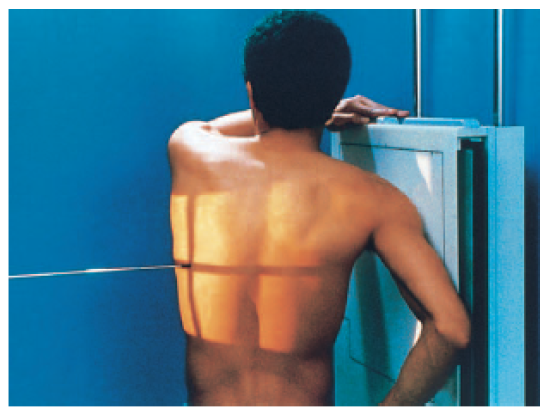
\includegraphics[width=1\linewidth]{imagenes/OA costillas.png}
    \caption{Proyección PA, OAD}
    \label{fig:g5}
\end{figure}

\subsubsection*{Rayo Central}
Perpendicular al receptor. Punto de entrada: \textbf{T7}, aproximadamente 8--10~cm por debajo de la escotadura yugular o al nivel correspondiente a la vértebra prominente (C7) contando hacia abajo. Centrado en la mitad de la región.

\subsubsection*{Receptor de imagen}
Centrado en el hemitórax de interés. Debe incluir desde los vértices pulmonares hasta los ángulos costofrénicos. Borde superior ubicado 4~cm por encima del borde superior del hombro para asegurar inclusión completa de los arcos superiores.

\subsubsection*{Respiración}
\begin{itemize}
  \item \textbf{Costillas supradiafragmáticas:} suspender al final de una \textbf{inspiración profunda} para desplazar el diafragma hacia abajo y liberar la mayor cantidad de arcos costales.
  \item \textbf{Costillas infradiafragmáticas:} suspender al final de una \textbf{espiración profunda} para elevar el diafragma y desenmascarar los arcos inferiores.
\end{itemize}

% ----- SECCIÓN 4 -----
\subsubsection*{4. Anatomía Visible}

\begin{itemize}
  \item \textbf{Porción axilar de los arcos costales} del lado de interés, desplegada y libre de superposición con la columna vertebral.
  \item Cortical ósea de los arcos costales visible de extremo a extremo.
  \item Costillas visibles a través del parénquima pulmonar (supradiafragmáticas) o a través del abdomen (infradiafragmáticas).
  \item La OAI despliega con mayor nitidez el \textbf{borde axilar derecho}.
  \item La OAD despliega con mayor nitidez el borde axilar izquierdo y puede complementarse para ver porciones \textbf{anteriores y mediales} del lado izquierdo.
\end{itemize}

% ----- SECCIÓN 5 -----
\subsubsection*{5. Criterios de Evaluación}

\textbf{Posicionamiento correcto:} la porción axilar de los arcos costales del lado afectado se proyecta libre de superposición. La distancia entre la columna vertebral y el borde lateral de las costillas del lado alejado es aproximadamente el doble de la del lado apoyado.\\

\textbf{Ausencia de exceso de rotación:} a nivel de los cuerpos vertebrales, el borde de cada cuerpo debe ser único y nítido; si se visualiza un doble borde, el paciente está rotado más allá de 45° (casi en perfil). La escápula y el húmero del lado alejado no deben proyectarse sobre el campo pulmonar.\\

\textbf{Inspiración correcta (supradiafragmáticas):} deben visualizarse entre 8 y 9 arcos costales posteriores por encima del diafragma, con las costillas anteriores de la 5.ª a la 7.ª visibles en su totalidad por encima del hemidiafragma correspondiente.\\

\textbf{Penetración y contraste:} las costillas deben ser visibles a través del parénquima pulmonar con contraste suficiente para distinguir la cortical ósea sin que la densidad del aire la borre. Técnica de alto contraste (kVp reducido).

% ----- SECCIÓN 6 -----
\subsubsection*{6. Puntos Críticos}

\textbf{Brazo del lado alejado mal posicionado:} si el brazo no se eleva correctamente, el húmero y la escápula se proyectan sobre los pulmones y ocluyen la región de interés. Pedir al paciente que tome la parte superior del Bucky o que eleve el brazo hasta la altura del hombro como mínimo.\\

\textbf{Exceso de rotación:} rotar más de 45° lleva al paciente casi a un perfil lateral, perdiendo la visión característica de la oblicua. El signo en la imagen es la doble sombra del cuerpo vertebral. Corregir reduciendo la rotación hasta 45° exactos.\\

\textbf{Confusión de nomenclatura OAD/OAI:} recordar que el nombre indica el lado que \emph{apoya} contra el receptor, no el lado que se estudia. La OAI (lado izquierdo apoyado) despliega el lado \textbf{derecho}; la OAD (lado derecho apoyado) despliega el lado \textbf{izquierdo}.\\

\textbf{Adaptaciones:} en pacientes con trauma severo que no pueden bipedestarse, realizar la oblicua en decúbito semiprono con el mismo ángulo de 45° asistido por cuñas de posicionamiento.\\

\textbf{Truco para porción anterior y medial:} si la oblicua estándar no despliega bien la porción más anterior y medial del arco costal, agregar una segunda oblicua del \emph{mismo lado afectado} (acercando el lado afectado al receptor en lugar de alejarlo). Ejemplo: trauma derecho $\rightarrow$ OAI (borde axilar) + OAD (porción anterior-medial).

\clearpage

\begin{figure}
    \centering
    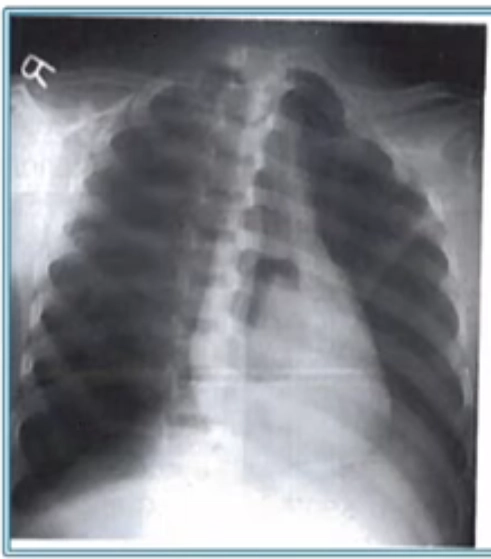
\includegraphics[width=0.5\linewidth]{imagenes/OAD costillas .png}
    \caption{Oblicua Anterior Derecha para ver el LADO IZQUIERDO}
    \label{fig:42}
\end{figure}

\begin{figure}
    \centering
    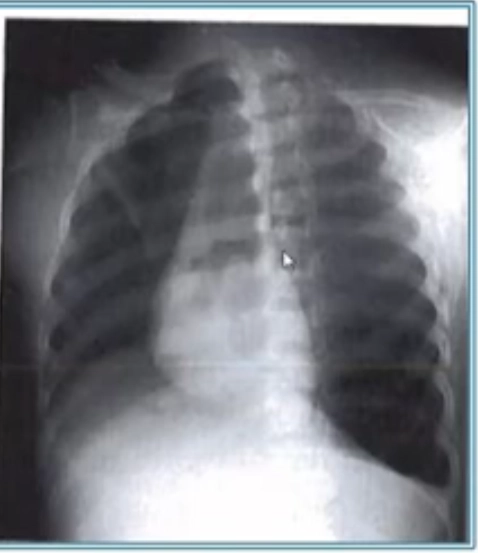
\includegraphics[width=0.5\linewidth]{imagenes/OAI costillas.png}
    \caption{Oblicua Anterior Izquierda para ver el LADO DERECHO}
    \label{fig:afadsf}
\end{figure}

\clearpage

% ============================================================
%  EJERCICIO CLÍNICO — Oblicuas de Parrilla Costal
% ============================================================

\subsubsection*{Ejercicio Clínico}

\noindent\textbf{DC:} Paciente con traumatismo costal, dolor en el reborde costal derecho superior irradiando hacia adelante.

\medskip
\noindent\textbf{Enfoques indicados:}

\begin{itemize}
  \item Radiografía de tórax PA estándar (estudio inicial obligatorio).
  \item \textbf{OAI} --- para desplegar el \textbf{borde axilar derecho} (lado afectado alejado del receptor).
  \item \textbf{OAD} --- complementaria, para desplegar la \textbf{porción anterior y medial del lado derecho} (lado afectado apoyado contra el receptor, mayor nitidez).
\end{itemize}

\medskip
\noindent\textbf{Nota anatómica:} la región \textbf{axilar} corresponde al borde externo de los arcos costales; la región \textbf{medial} corresponde a la zona próxima al esternón.

\medskip
\noindent\textbf{Regla fundamental:} en las oblicuas anteriores, \emph{siempre se despliega el lado contrario al que apoya contra el receptor}.

\medskip
\noindent\textbf{Colimación:} se colima al \textbf{hemitórax de interés} únicamente. A diferencia de las oblicuas indicadas para corazón y grandes vasos, en el estudio de parrilla costal no es necesario incluir todo el tórax.

\clearpage

\begin{figure}
    \centering
    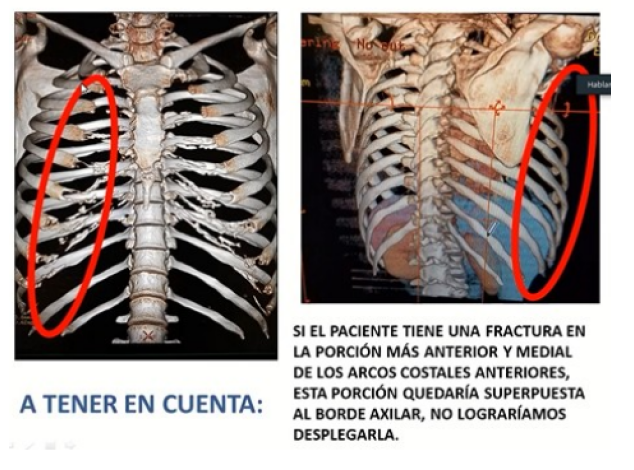
\includegraphics[width=0.65\linewidth]{imagenes/oblicuas costales ejercicio.png}
    \caption{}
    \label{fig:3334}
\end{figure}

\begin{figure}
    \centering
    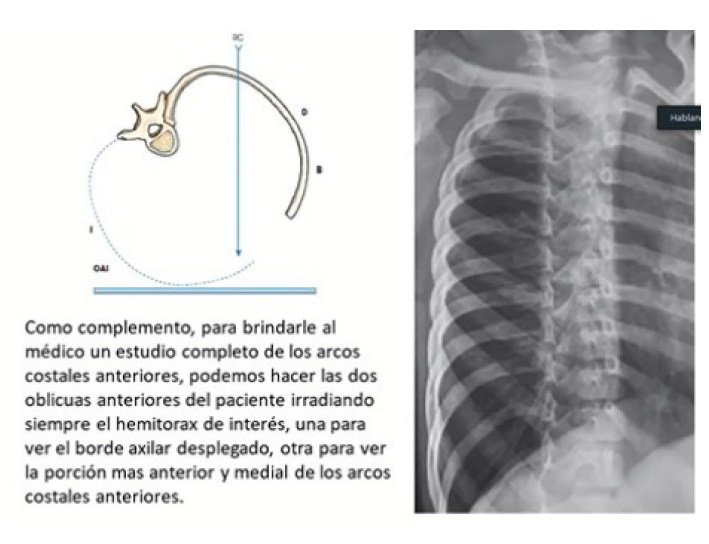
\includegraphics[width=0.65\linewidth]{oblicuas costales ejercicio 2.png}
    \caption{}
    \label{fig:g5w}
\end{figure}

\clearpage

% ============================================================
%  RESUMEN — Proyección AP Oblicua Posterior de Parrilla Costal
%           Porción Axilar (OPD / OPI)
% ============================================================

\subsection{Tórax - AP Oblicua Posterior de Parrilla Costal (OPD / OPI)}

% ----- SECCIÓN 1 -----
\subsubsection*{1. Identificación}

\textbf{Tipo:} Proyección complementaria. Forma parte de la serie de oblicuas de parrilla costal; siempre acompañada de una radiografía de tórax PA estándar previa. Se indica cuando el mecanismo de trauma es posterior o axilar posterior (caída de costado hacia atrás).\\

\textbf{Indicaciones clínicas principales:}

\begin{itemize}
  \item Traumatismo costal con dolor en el borde axilar posterior.
  \item Sospecha de fractura o fisura de arcos costales posteriores.
  \item Caída de costado hacia atrás con dolor axilar y dorsal localizado.
  \item Lesiones costales posteriores no evaluables en proyección frontal por superposición.
\end{itemize}

% ----- SECCIÓN 2 -----
\subsubsection*{2. Técnica Base}

\textbf{Receptor de imagen:} 35 $\times$ 43~cm. Orientación \textbf{longitudinal} respecto al eje mayor de la región. Borde superior 2~cm por encima de la vértebra prominente (C7).\\

\textbf{DFRI:} 100~cm.\\

\textbf{Técnica:} básica o intermedia para paciente estándar. Interés óseo: kVp reducido para alto contraste, permitiendo visualizar la cortical de los arcos costales posteriores con nitidez a través del parénquima pulmonar o del abdomen según la región estudiada.\\

\textbf{Bucky:} sí, Bucky mural.

% ----- SECCIÓN 3 -----
\subsubsection*{3. Posicionamiento}

\subsubsection*{Paciente}
Bipedestación con la espalda orientada hacia el receptor (posición AP), o decúbito supino si el paciente no puede mantenerse de pie. El plano medio sagital forma un ángulo de \textbf{45°} con el plano del RI. A diferencia de las oblicuas anteriores, en las posteriores el \textbf{lado afectado se acerca} al receptor.

\subsubsection*{Región de interés}
El cuerpo rota 45° apoyando el hombro posterior del lado afectado contra el RI:

\begin{itemize}
  \item \textbf{OPI} (para arcos costales izquierdos): el lado izquierdo es el afectado; el hombro posterior izquierdo se apoya contra el RI.
  \item \textbf{OPD} (para arcos costales derechos): el lado derecho es el afectado; el hombro posterior derecho se apoya contra el RI.
\end{itemize}

Posición de los brazos:
\begin{itemize}
  \item \textbf{Brazo del lado afectado} (más cercano al receptor): elevado con la mano apoyada sobre la cabeza, para retirar el húmero y la escápula del campo de interés.
  \item \textbf{Brazo contralateral} (alejado del receptor): abducido con la mano en la cadera.
\end{itemize}

\begin{figure}
    \centering
    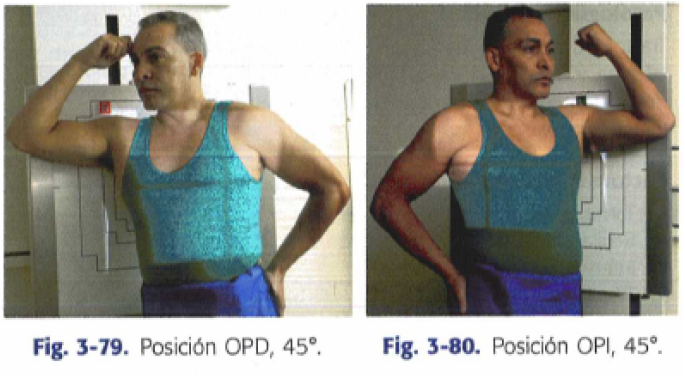
\includegraphics[width=1\linewidth]{imagenes/OP costales.png}
    \caption{}
    \label{fig:adsf}
\end{figure}


\subsubsection*{Rayo Central}
Perpendicular al receptor. Punto de entrada: \textbf{T7}, aproximadamente 8--10~cm por debajo de la escotadura yugular. Centrado en la mitad de la región de interés.

\subsubsection*{Receptor de imagen}
Centrado en el hemitórax de interés. Debe incluir desde los vértices costales hasta los ángulos costofrénicos. Borde superior posicionado 2~cm por encima de la vértebra prominente (C7) para asegurar la inclusión de los arcos superiores. Se colima al hemitórax de interés, sin necesidad de incluir todo el tórax.

\subsubsection*{Respiración}
\begin{itemize}
  \item \textbf{Costillas supradiafragmáticas:} suspender al final de una \textbf{inspiración profunda} para desplazar el diafragma caudalmente y liberar los arcos costales.
  \item \textbf{Costillas infradiafragmáticas:} suspender al final de una \textbf{espiración profunda} para elevar el diafragma y desenmascarar los arcos inferiores.
\end{itemize}

% ----- SECCIÓN 4 -----
\subsubsection*{4. Anatomía Visible}

\begin{itemize}
  \item \textbf{Porción axilar de los arcos costales posteriores} del lado afectado, desplegada y libre de superposición con la columna vertebral. Las costillas deben verse alargadas en su recorrido.
  \item Perfil de la \textbf{tráquea} lleno de aire, visible como columna radiolúcida central.
  \item Cortical ósea de los arcos costales visible de extremo a extremo, a través del parénquima pulmonar (supradiafragmáticas) o del abdomen (infradiafragmáticas).
  \item \textbf{Escápula del lado afectado} desplazada lateralmente, fuera del campo costal, sin superponerse al borde externo de las costillas.
  \item \textbf{OPD:} visualiza arcos costales derechos y borde axilar derecho. Las porciones anteriores y mediales se ven con longitud reducida pero con mayor definición, útiles para evaluar fracturas en esa zona.
  \item \textbf{OPI:} visualiza arcos costales izquierdos y borde axilar izquierdo.
  \item Distancia entre la columna vertebral y el borde lateral de las costillas del lado afectado aproximadamente el doble respecto al lado contralateral.
\end{itemize}

% ----- SECCIÓN 5 -----
\subsubsection*{5. Criterios de Evaluación}

\textbf{Posicionamiento correcto:} la porción axilar de los arcos costales del lado afectado se proyecta libre de superposición. Las costillas se ven \textbf{alargadas}, con su curvatura desplegada. La distancia columna--borde lateral costal del lado afectado es el doble de la del lado contralateral. Los hombros deben estar nivelados horizontalmente.\\

\textbf{Ausencia de exceso de rotación:} si el paciente rota más de 45° las costillas se \textbf{acortan} y muestran una curvatura cerrada sobre sí mismas (aspecto casi de perfil). Adicionalmente, la columna comienza a proyectarse sobre el parénquima del hemitórax de interés, ocultando estructuras. Corregir reduciendo la rotación a 45° exactos.\\

\textbf{Posición correcta de la escápula:} la escápula del lado afectado debe estar desplazada hacia lateral, sin superponerse al borde externo costal. Si se superpone, el brazo no fue elevado correctamente.\\

\textbf{Marca del mismo lado que las apófisis espinosas:} en las oblicuas posteriores, las apófisis espinosas y la marca del lado apoyado coinciden en el mismo hemitórax (equivalencia OPD $\approx$ OAI; OPI $\approx$ OAD).\\

\textbf{Penetración y contraste:} las costillas posteriores deben ser visibles a través del parénquima pulmonar con contraste suficiente para distinguir la cortical ósea. Técnica de alto contraste (kVp reducido).

% ----- SECCIÓN 6 -----
\subsubsection*{6. Puntos Críticos}

\textbf{Brazo del lado afectado mal posicionado:} si el brazo no se eleva con la mano sobre la cabeza, la escápula se proyecta sobre el campo costal y oscurece la región de interés. Es el error más frecuente en esta proyección.\\

\textbf{Exceso de rotación:} más de 45° produce el acortamiento de las costillas y la superposición de la columna sobre el hemitórax afectado. El signo en imagen es la curvatura cerrada de los arcos y la columna cubriendo el parénquima derecho o izquierdo según el lado estudiado. Reducir la rotación y verificar que los hombros queden nivelados.\\

\textbf{Confusión con las oblicuas anteriores:} en las oblicuas posteriores el lado afectado \emph{se acerca} al receptor (al contrario de las anteriores). Recordar: \textbf{AP oblicua posterior = acerco el lado afectado}; \textbf{PA oblicua anterior = alejo el lado afectado}.\\

\textbf{Equivalencia con oblicuas anteriores:} OPI $\approx$ OAD (cuerpos vertebrales mirando hacia la izquierda del observador); OPD $\approx$ OAI (cuerpos vertebrales mirando hacia la derecha del observador). Esta equivalencia es útil para verificar el posicionamiento comparando con estudios previos.\\

\textbf{Adaptaciones:} en pacientes que no pueden bipedestarse, realizar la oblicua en decúbito supino con cuña de posicionamiento a 45° bajo el lado no afectado para lograr la rotación equivalente.\\

\textbf{Colimación:} colimar al hemitórax de interés exclusivamente. A diferencia de las oblicuas para corazón y grandes vasos, no es necesario incluir todo el tórax.

\clearpage

\begin{figure}
    \centering
    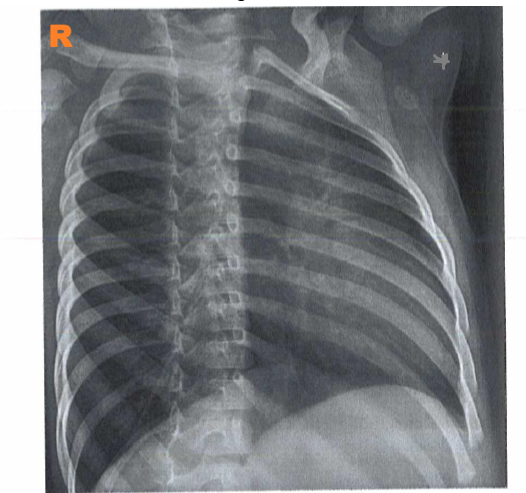
\includegraphics[width=1\linewidth]{imagenes/OP costales 2.png}
    \caption{Marca del mismo lado que las apófisis espinosas / Cuerpos vertebrales hacia la derecha del observador (OAD/OPI)}
    \label{fig:342314}
\end{figure}


% ============================================================
%  INTERPRETACIÓN DE IMAGEN — Identificación de Oblicuas
% ============================================================

\subsubsection*{Interpretación de Imagen: Identificación de la Oblicua}

\noindent
Ante una imagen oblicua de parrilla costal, la identificación completa del enfoque tiene dos pasos independientes: determinar \textbf{qué lado se desplegó} y determinar \textbf{si la oblicua es anterior o posterior}.

\medskip
\noindent\textbf{Paso 1 --- Determinar el lado desplegado.}
Observar hacia qué lado se desplazó la columna vertebral y cuál es el hemitórax con los arcos costales desplegados: ese es el lado de interés. Recordar que la \textbf{derecha del paciente siempre queda a nuestra izquierda} en la imagen. Ejemplo: si la columna se corrió hacia la derecha del observador y los arcos izquierdos están desplegados (con la silueta cardíaca visible), el lado estudiado es el \textbf{izquierdo}.

\medskip
\noindent\textbf{Paso 2 --- Determinar si es anterior o posterior.}
\textbf{No es posible diferenciar una oblicua anterior de una posterior} únicamente por la imagen. Una OAD y una OPI producen una imagen equivalente: ambas despliegan el lado izquierdo. La distinción requiere conocer el mecanismo de trauma o disponer de los datos clínicos del estudio.

\begin{itemize}
  \item \textbf{OAD} (oblicua anterior derecha) $\equiv$ despliega el lado izquierdo.
  \item \textbf{OPI} (oblicua posterior izquierda) $\equiv$ despliega el lado izquierdo.
  \item Ambas producen una imagen radiológicamente indistinguible.
\end{itemize}

\medskip
\noindent\textbf{Adaptación según contextura del paciente.}
El ángulo de rotación de 45° es el estándar, pero debe ajustarse según el diámetro del paciente:

\begin{itemize}
  \item \textbf{Paciente con gran diámetro anteroposterior:} rotar \emph{menos} de 45°; la mayor masa corporal ya proyecta suficientemente el lado lateral de interés.
  \item \textbf{Paciente delgado:} rotar \emph{más} de 45° para lograr el mismo efecto de despliegue costal.
\end{itemize}

\begin{figure}[h]
    \centering
    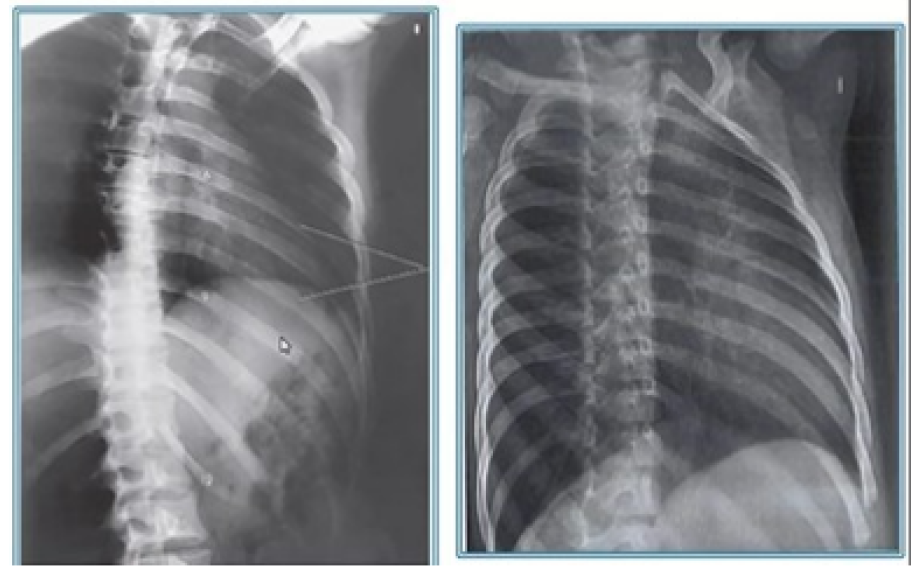
\includegraphics[width=1\linewidth]{imagenes/OP costales 3.png}
    \caption{Enter Caption}
    \label{fig:hysh}
\end{figure}